\documentclass[hyperref={bookmarks=false},aspectratio=169]{beamer}
\usepackage{hyperref,ragged2e,amsmath,amssymb,url,bm}
\usepackage{graphicx,booktabs,array}
\usepackage{tikz}
\usetikzlibrary{arrows.meta,positioning,calc,shapes.geometric,decorations.pathreplacing,matrix}
\graphicspath{{crops/}}
\usetheme{Goettingen}
% --- Paleta: azul profundo, dorado y papiro crema ---
\definecolor{azul}{HTML}{15437C}
\definecolor{azuloscuro}{HTML}{0B1F3A}
\definecolor{celeste}{HTML}{5694D6}
\definecolor{dorado}{RGB}{196,154,60}
\definecolor{papiro}{RGB}{246,239,220}
\definecolor{gris}{RGB}{70,78,96}
\setbeamercolor{structure}{fg=azul}
\setbeamertemplate{sidebar canvas right}[vertical shading][top=azul,bottom=azuloscuro]
\setbeamercolor{title in sidebar}{fg=dorado}
\setbeamercolor{author in sidebar}{fg=papiro}
\setbeamercolor{section in sidebar}{fg=papiro}
\setbeamercolor{section in sidebar shaded}{fg=dorado!70!papiro}
\setbeamercolor{subsection in sidebar}{fg=papiro}
\setbeamercolor{subsection in sidebar shaded}{fg=dorado!70!papiro}
\let\raggedright\justifying
\setlength{\RaggedRightRightskip}{0pt plus 1fil}
\setbeamertemplate{background canvas}{
\includegraphics[width=\paperwidth,height=\paperheight]{papiro.jpg}}
\setbeamercolor{normal text}{fg=black!88!azuloscuro}
\setbeamercolor{frametitle}{fg=azul}
\setbeamerfont{frametitle}{series=\bfseries}
\setbeamertemplate{section in toc shaded}{\leavevmode{\color{gris}\inserttocsection}\par}
\setbeamercolor{title}{fg=azul}
\setbeamercolor{subtitle}{fg=gris}
\setbeamercolor{item projected}{bg=azul,fg=papiro}
\setbeamertemplate{itemize item}{\small\textcolor{dorado}{$\blacktriangleright$}}
\setbeamertemplate{navigation symbols}{}
% --- Español + hebreo + griego (XeLaTeX) ---
\usepackage[bidi=default]{babel}
\babelprovide[import,main]{spanish}
\babelprovide[import]{hebrew}
\babelprovide[import]{ancientgreek}
\babelfont[hebrew]{sf}[Path=fonts/, BoldFont=NotoHebrewSans-700.ttf]{NotoHebrewSans-400.ttf}
\babelfont[hebrew]{rm}[Path=fonts/, BoldFont=NotoHebrewSans-700.ttf]{NotoHebrewSans-400.ttf}
\babelfont[ancientgreek]{sf}[Path=fonts/]{GFSPorson.otf}
\babelfont[ancientgreek]{rm}[Path=fonts/]{GFSPorson.otf}
\newcommand{\heb}[1]{\mbox{\foreignlanguage{hebrew}{#1}}}
\newcommand{\grc}[1]{\foreignlanguage{ancientgreek}{#1}}
\newcommand{\SENOR}{S{\fontsize{0.78em}{1em}\selectfont EÑOR}}
% --- Citas (cuadro de un solo color), imágenes, referencias ---
\usepackage[most]{tcolorbox}
\newtcolorbox{cita}[1][]{enhanced, colback=azul!7!papiro, opacityback=0.85, colframe=azul,
  boxrule=0pt, leftrule=2.5pt, arc=0pt, left=6pt, right=6pt, top=4pt, bottom=4pt,
  before skip=4pt, after skip=6pt, fontupper=\small\itshape, #1}
\newcommand{\fuente}[1]{\par\hfill{\upshape\bfseries\footnotesize\textcolor{azul}{#1}}}
\makeatletter
\newcommand{\fotolado}[2]{%
  \begin{tikzpicture}[remember picture,overlay]
    \node[anchor=north east,inner sep=0pt] (foto) at ([xshift=-\beamer@sidebarwidth]current page.north east)
      {\includegraphics[height=\paperheight]{#1}};
    \node[anchor=south east,inner sep=2pt,text=papiro,fill=azuloscuro,fill opacity=0.6,text opacity=1,
      font=\fontsize{4.5}{5.5}\selectfont,align=right,text width=4.2cm] at ([xshift=-3pt,yshift=3pt]foto.south east)
      {\textit{Nota.} #2};
  \end{tikzpicture}}
\makeatother
\newcommand{\refapa}[1]{\par{\RaggedRight\hangindent=1.2em\hangafter=1\noindent #1\par}\vspace{3pt}}
\usepackage{xurl}\urlstyle{same}
\newcommand{\destacar}[1]{\textbf{\textcolor{azul}{#1}}}
\newcommand{\precision}[1]{{\footnotesize\color{gris}\textbf{Precisión:} #1}}
\tikzset{caja/.style={draw=azul,line width=0.8pt,fill=papiro,fill opacity=0.92,text opacity=1,rounded corners=3pt,inner sep=5pt,font=\scriptsize}}
\title[El celo de Dios]{\bfseries{El celo de Dios}}
\subtitle{``\SENOR, cuyo nombre es Celoso, Dios celoso es'' (Éx 34:14)}
\author{}\institute{}\date{}
\titlegraphic{
\includegraphics[width=0.80\linewidth,height=0.36\textheight,keepaspectratio]{portada.jpg}\\[-1pt]
  {\fontsize{5}{6}\selectfont\color{gris}\textit{Nota.} Elaboración propia: Éx 34:14b en texto hebreo consonántico (BHS).}}
\begin{document}
\frame{\titlepage}


% ------------------------------------------------------------------
\section{Contexto}

\begin{frame}{Una palabra incómoda}
\begin{columns}[c,onlytextwidth]
\begin{column}{0.50\textwidth}
\begin{cita}Porque los celos son el furor del hombre, Y no perdonará en el día de la venganza. No aceptará ningún rescate, Ni querrá perdonar, aunque multipliques los dones.\fuente{(Pr 6:34--35, RVR1960)}\end{cita}
\begin{center}\heb{כִּי־קִנְאָה חֲמַת־גָּבֶר}\end{center}
\scriptsize ``Porque el celo (\emph{qin'á}) es el ardor (\emph{jamat}) del varón'': el marido ofendido no acepta rescate.
\end{column}
\begin{column}{0.48\textwidth}\small
\begin{itemize}
\item En nuestra cultura, ``celos'' suena a \destacar{inseguridad}, posesión, desconfianza.
\item Proverbios lo usa como \destacar{ilustración humana}: el esposo traicionado no negocia la exclusividad del pacto.
\item Dios dice de sí mismo: ``\SENOR, cuyo nombre es \destacar{Celoso}'' (Éx 34:14).
\item ¿Cómo puede ser perfección eterna algo que en nosotros suele ser defecto?
\end{itemize}
\end{column}
\end{columns}
\precision{Pr 6:34--35 describe el celo humano; sirve de ilustración, no de definición del celo de Dios.}
\end{frame}

\begin{frame}{Cuatro preguntas}
\centering
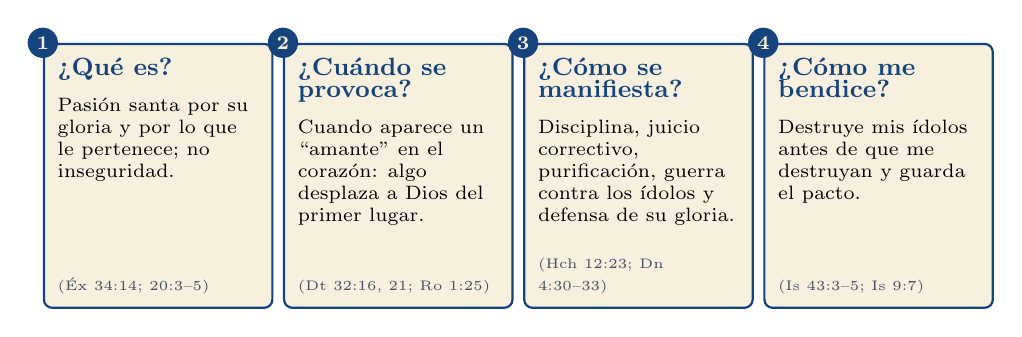
\begin{tikzpicture}
 \foreach \x/\n/\t/\d/\r in {0/1/{¿Qué es?}/{Pasión santa por su gloria y por lo que le pertenece; no inseguridad.}/{Éx 34:14; 20:3--5},
   3.05/2/{¿Cuándo se provoca?}/{Cuando aparece un ``amante'' en el corazón: algo desplaza a Dios del primer lugar.}/{Dt 32:16, 21; Ro 1:25},
   6.1/3/{¿Cómo se manifiesta?}/{Disciplina, juicio correctivo, purificación, guerra contra los ídolos y defensa de su gloria.}/{Hch 12:23; Dn 4:30--33},
   9.15/4/{¿Cómo me bendice?}/{Destruye mis ídolos antes de que me destruyan y guarda el pacto.}/{Is 43:3--5; Is 9:7}}{
  \node[caja,anchor=north] (b\n) at (\x,0) {\parbox[t][3.0cm][t]{2.55cm}{\RaggedRight
    {\small\textbf{\textcolor{azul}{\t}}}\\[5pt]\scriptsize \d\par\vfill{\tiny\color{gris}(\r)}}};
  \node[circle,fill=azul,text=papiro,font=\scriptsize\bfseries,inner sep=1.6pt] at (b\n.north west) {\n};}
\end{tikzpicture}\par\medskip
\small\RaggedRight Las cuatro preguntas de tu sermón ordenan el estudio. A ellas se suman dos que pediste desarrollar: qué dice exactamente \destacar{Éxodo} (sustantivo o adjetivo) y por qué \destacar{Isaías 9} atribuye al celo de Dios la venida del Mesías.
\end{frame}

\begin{frame}{Un atributo de relación}
\begin{columns}[c,onlytextwidth]
\begin{column}{0.50\textwidth}
\centering
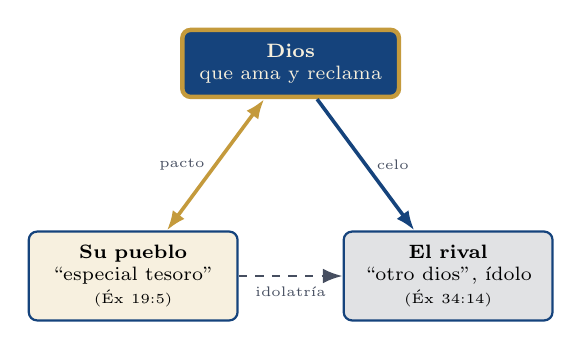
\begin{tikzpicture}[font=\scriptsize]
 \node[draw=dorado,line width=1.6pt,fill=azul,text=papiro,rounded corners=3pt,text width=2.4cm,align=center,inner sep=5pt] (d) at (0,1.9) {\textbf{Dios}\\ que ama y reclama};
 \node[caja,text width=2.3cm,align=center] (p) at (-2.0,-0.8) {\textbf{Su pueblo}\\ ``especial tesoro''\\ {\tiny(Éx 19:5)}};
 \node[caja,text width=2.3cm,align=center,fill=gris!18] (r) at (2.0,-0.8) {\textbf{El rival}\\ ``otro dios'', ídolo\\ {\tiny(Éx 34:14)}};
 \draw[{Latex[length=2.5mm]}-{Latex[length=2.5mm]},dorado,line width=1.3pt] (d)--(p) node[midway,left,font=\tiny,text=gris]{pacto};
 \draw[-{Latex[length=2.5mm]},gris,line width=1pt,dashed] (p)--(r) node[midway,below,font=\tiny,text=gris]{idolatría};
 \draw[-{Latex[length=2.5mm]},azul,line width=1.3pt] (d)--(r) node[midway,right,font=\tiny,text=gris]{celo};
\end{tikzpicture}
\end{column}
\begin{column}{0.48\textwidth}\small
\begin{itemize}
\item El celo necesita \destacar{tres términos}: alguien que ama, alguien amado que le pertenece y un rival.
\item Por eso es un atributo de \destacar{relación}: se revela en el pacto. Sin pueblo no hay celo; sin ídolo no se enciende.
\item Pero no es una reacción nueva en Dios: es su \destacar{santo amor} de siempre, visto desde el lado de la exclusividad.
\end{itemize}
\end{column}
\end{columns}\par\smallskip
\precision{clasificación propuesta: atributo de Relación; \emph{incomunicable} en su derecho (solo Dios puede exigir adoración exclusiva), \emph{comunicable} como reflejo (el ``celo por Dios'' de Pinjás, Elías y Pablo).}
\end{frame}

\begin{frame}{``Celo'' en la Biblia}
\begin{columns}[c,onlytextwidth]
\begin{column}{0.40\textwidth}\footnotesize
\begin{itemize}
\item RVR1960: ``celo, celos, celoso, celar'' \textbf{91 veces} en \textbf{78 versículos} (64 AT, 27 NT).
\item Hebreo: la raíz \heb{קנא} aparece \textbf{85 veces} en \textbf{70 versículos}.
\item Griego NT: la familia \grc{ζῆλος} aparece \textbf{40 veces} en \textbf{38 versículos}.
\item La misma raíz se traduce ``celo'' y también ``\destacar{envidia}''.
\end{itemize}
\end{column}
\begin{column}{0.58\textwidth}
\scriptsize\renewcommand{\arraystretch}{1.12}
\begin{tabular}{@{}>{\RaggedRight\arraybackslash}p{3.5cm}>{\RaggedRight\arraybackslash}p{2.3cm}r@{}}
\toprule
\textbf{Término} & \textbf{Sentido base} & \textbf{Veces} \\ \midrule
\heb{קִנְאָה} \emph{qin'á} (sust.) & celo, celos, envidia & 44 \\
\heb{קִנֵּא} \emph{qinné}, \heb{הִקְנִיא} \emph{hiqní} (verbo) & tener celo; provocar a celos & 33 \\
\heb{קַנָּא} \emph{qanná} (adj.) & celoso (solo Dios) & 6 \\
\heb{קַנּוֹא} \emph{qannó} (adj.) & celoso (solo Dios) & 2 \\ \midrule
\grc{ζῆλος} \emph{zēlos} & celo, ardor, envidia & 16 \\
\grc{ζηλόω} \emph{zēlóō} & celar, procurar & 12 \\
\grc{ζηλωτής} \emph{zēlōtēs} & celoso, zelote & 8 \\
\grc{παραζηλόω} \emph{parazēlóō} & provocar a celos & 4 \\
\bottomrule
\end{tabular}
\end{column}
\end{columns}\par\smallskip
\precision{conteo propio (RVR1960 sin títulos de sección; BHS y NA27 con Strong). Vine da 43 para el sustantivo y 34 para el verbo; el total, 85, coincide. Verificar en e-Sword.}
\end{frame}

% ------------------------------------------------------------------
\section{Éxodo}

\begin{frame}{El segundo mandamiento}
\begin{columns}[c,onlytextwidth]
\begin{column}{0.52\textwidth}
\begin{cita}No tendrás dioses ajenos delante de mí. No te harás imagen, ni ninguna semejanza\ldots{} No te inclinarás a ellas, ni las honrarás; porque yo soy \SENOR{} tu Dios, fuerte, celoso, que visito la maldad de los padres sobre los hijos hasta la tercera y cuarta generación de los que me aborrecen.\fuente{(Éx 20:3--5, RVR1960)}\end{cita}
\end{column}
\begin{column}{0.46\textwidth}
\begin{center}\heb{כִּי אָנֹכִי יְהוָה אֱלֹהֶיךָ אֵל קַנָּא}\end{center}
\scriptsize\renewcommand{\arraystretch}{1.15}
\begin{tabular}{@{}>{\RaggedRight\arraybackslash}p{1.9cm}>{\RaggedRight\arraybackslash}p{3.7cm}@{}}
\toprule
\heb{אֵל} \emph{El} & ``Dios''; la RVR1960 traduce ``fuerte''. \\
\heb{קַנָּא} \emph{qanná} & adjetivo: ``celoso''. Califica a \emph{El}. \\
\heb{עַל־פָּנָי} & ``delante de mí'', literalmente ``sobre mi rostro'': ningún dios en mi presencia. \\
\bottomrule
\end{tabular}\par\smallskip
\small El primer uso del adjetivo en la Biblia justifica el mandamiento: Dios no comparte la adoración.
\end{column}
\end{columns}
\end{frame}

\begin{frame}{Texto ancla: Éx 34:12--14}
\fotolado{panel_exodo34.jpg}{Elaboración propia: Éx 34:14 en texto hebreo consonántico (BHS).}
\begin{columns}[c,onlytextwidth]
\begin{column}{0.58\textwidth}
\begin{cita}Guárdate de hacer alianza con los moradores de la tierra donde has de entrar, para que no sean tropezadero en medio de ti. Derribaréis sus altares, y quebraréis sus estatuas, y cortaréis sus imágenes de Asera. Porque no te has de inclinar a ningún otro dios, pues \SENOR, cuyo nombre es Celoso, Dios celoso es.\fuente{(Éx 34:12--14, RVR1960)}\end{cita}
\small El pacto se renueva después del becerro de oro (Éx 32). En el mismo capítulo, Dios proclama su nombre ``misericordioso y piadoso'' (34:6) y declara que su nombre es ``Celoso'' (34:14).
\end{column}
\begin{column}{0.40\textwidth}\end{column}
\end{columns}
\end{frame}

\begin{frame}{¿Sustantivo o adjetivo?}
\begin{center}\large\heb{כִּי יְהוָה קַנָּא שְׁמוֹ אֵל קַנָּא הוּא}\end{center}
\scriptsize\renewcommand{\arraystretch}{1.15}
\begin{tabular}{@{}>{\RaggedRight\arraybackslash}p{2.0cm}>{\RaggedRight\arraybackslash}p{2.6cm}>{\RaggedRight\arraybackslash}p{7.2cm}@{}}
\toprule
\textbf{Hebreo} & \textbf{Función} & \textbf{Sentido} \\ \midrule
\heb{יְהוָה} & sujeto & ``el \SENOR'' (el Nombre, \emph{Adonay}). \\
\heb{קַנָּא שְׁמוֹ} \emph{qanná shemó} & \emph{qanná} usado \destacar{como nombre} & ``Celoso (es) su nombre'': el adjetivo funciona como sustantivo, un nombre propio. La RVR1960 lo escribe con mayúscula. \\
\heb{אֵל קַנָּא הוּא} \emph{El qanná hu} & \emph{qanná} \destacar{como adjetivo} & ``Dios celoso (es) él'': califica a \emph{El}, como en Éx 20:5. \\
\bottomrule
\end{tabular}\par\medskip
\begin{columns}[t,onlytextwidth]
\begin{column}{0.49\textwidth}\small
\textbf{Verificación:} tu intuición es correcta en la función, con un matiz: es \destacar{la misma palabra}, \emph{qanná}, dos veces. La primera como nombre (sustantivada); la segunda como adjetivo. El sustantivo propiamente dicho, \heb{קִנְאָה} \emph{qin'á} (``celo''), no aparece en Éx 20 ni en Éx 34.
\end{column}
\begin{column}{0.49\textwidth}\scriptsize
\textbf{LXX:} \grc{ὁ γὰρ κύριος ὁ θεὸς ζηλωτὸν ὄνομα, θεὸς ζηλωτής ἐστιν}: ``el Señor Dios es nombre celoso, Dios celoso es''.\par\smallskip
\textbf{Ónkelos:} \heb{אֲרֵי יְיָ קַנָּא שְׁמֵיהּ אֵל קַנָּא הוּא}: conserva las dos palabras.\par\smallskip
\precision{el celo no es aquí una emoción pasajera sino un \emph{nombre}: identidad revelada (cf. Éx 3:15).}
\end{column}
\end{columns}
\end{frame}

\begin{frame}{``Celoso'': un adjetivo solo de Dios}
\begin{columns}[c,onlytextwidth]
\begin{column}{0.55\textwidth}
\scriptsize\renewcommand{\arraystretch}{1.12}
\begin{tabular}{@{}>{\RaggedRight\arraybackslash}p{1.6cm}>{\RaggedRight\arraybackslash}p{1.3cm}>{\RaggedRight\arraybackslash}p{3.6cm}@{}}
\toprule
\textbf{Texto} & \textbf{Forma} & \textbf{Contexto} \\ \midrule
Éx 20:5 & \heb{אֵל קַנָּא} & segundo mandamiento \\
Éx 34:14 (×2) & \heb{קַנָּא שְׁמוֹ} & ``otro dios''; Asera \\
Dt 4:24 & \heb{אֵל קַנָּא} & ``fuego consumidor'' \\
Dt 5:9 & \heb{אֵל קַנָּא} & mandamiento repetido \\
Dt 6:15 & \heb{אֵל קַנָּא} & ``no andaréis en pos de dioses ajenos'' \\
Jos 24:19 & \heb{אֵל־קַנּוֹא} & renovación del pacto en Siquem \\
Nah 1:2 & \heb{אֵל קַנּוֹא} & juicio contra Nínive \\
\bottomrule
\end{tabular}
\end{column}
\begin{column}{0.43\textwidth}\small
\begin{itemize}
\item Las 8 apariciones del adjetivo se refieren a \destacar{Dios}; ninguna a un ser humano.
\item Siempre van con \heb{אֵל} \emph{El}: ``Dios celoso''.
\item Siempre en el \destacar{pacto} y frente a la \destacar{idolatría}.
\item En Josué va junto a ``Dios \emph{santo}'' (\heb{קְדֹשִׁים}): el celo es la santidad que no tolera rivales.
\end{itemize}
\end{column}
\end{columns}
\end{frame}

\begin{frame}{Éxodo 34: misericordia y celo}
\centering
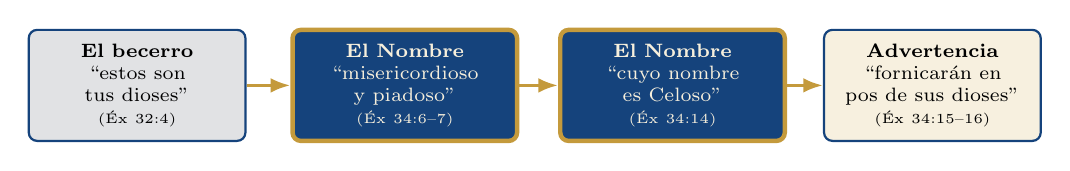
\begin{tikzpicture}[font=\scriptsize]
 \node[caja,text width=2.4cm,align=center,fill=gris!18] (a) at (0.2,0) {\textbf{El becerro}\\ ``estos son tus dioses''\\ {\tiny(Éx 32:4)}};
 \node[draw=dorado,line width=1.6pt,fill=azul,text=papiro,rounded corners=3pt,text width=2.5cm,align=center,inner sep=5pt] (b) at (3.6,0) {\textbf{El Nombre}\\ ``misericordioso y piadoso''\\ {\tiny(Éx 34:6--7)}};
 \node[draw=dorado,line width=1.6pt,fill=azul,text=papiro,rounded corners=3pt,text width=2.5cm,align=center,inner sep=5pt] (c) at (7.0,0) {\textbf{El Nombre}\\ ``cuyo nombre es Celoso''\\ {\tiny(Éx 34:14)}};
 \node[caja,text width=2.4cm,align=center] (d) at (10.3,0) {\textbf{Advertencia}\\ ``fornicarán en pos de sus dioses''\\ {\tiny(Éx 34:15--16)}};
 \draw[-{Latex[length=2.5mm]},dorado,line width=1.2pt] (a)--(b); \draw[-{Latex[length=2.5mm]},dorado,line width=1.2pt] (b)--(c); \draw[-{Latex[length=2.5mm]},dorado,line width=1.2pt] (c)--(d);
\end{tikzpicture}\par\medskip
\begin{columns}[t,onlytextwidth]
\begin{column}{0.49\textwidth}\small
\begin{itemize}
\item Dios no tiene dos caras: la misma revelación del Sinaí junta \destacar{misericordia} y \destacar{celo}.
\item El que perdona a Israel después del becerro es el que no tolerará otro becerro.
\end{itemize}
\end{column}
\begin{column}{0.49\textwidth}\scriptsize
La frase \heb{וְזָנוּ אַחֲרֵי אֱלֹהֵיהֶם} (\emph{vezanú ajaré eloheihem}) dice ``y fornicarán en pos de sus dioses''. \heb{זָנָה} \emph{zaná} es el verbo de la infidelidad conyugal. El pacto es un \destacar{matrimonio}; la idolatría, un adulterio. Por eso Dios es ``celoso''.
\end{column}
\end{columns}
\end{frame}

% ------------------------------------------------------------------
\section{La palabra}

\begin{frame}{La raíz: ardor}
\centering
\begin{tikzpicture}[font=\scriptsize]
 \node[draw=dorado,line width=1.6pt,fill=azul,text=papiro,rounded corners=3pt,text width=2.6cm,align=center,inner sep=6pt,font=\small\bfseries] (c) at (0,0) {CALOR};
 \node[caja,text width=3.0cm,align=center] (h) at (-4.3,1.3) {\textbf{Hebreo} \heb{קנא}\\ \emph{qaná}: arder de celo; el árabe \emph{qana'a}, ``enrojecer intensamente''};
 \node[caja,text width=3.0cm,align=center] (g) at (4.3,1.3) {\textbf{Griego} \grc{ζῆλος}\\ de \grc{ζέω}, ``hervir'': ``propiamente calor'' (Strong)};
 \node[caja,text width=3.0cm,align=center] (e) at (-4.3,-1.4) {\textbf{Español} ``celo''\\ del latín \emph{zelus}, y este del griego \emph{zêlos} (DLE)};
 \node[caja,text width=3.0cm,align=center] (p) at (4.3,-1.4) {\textbf{Par hebreo} \heb{חֵמָה}\\ \emph{jemá}: ``calor, furor''; acompaña a \emph{qin'á}};
 \foreach \i in {h,g,e,p}\draw[dorado,line width=1.1pt] (c)--(\i);
\end{tikzpicture}\par\medskip
\small\RaggedRight En las tres lenguas, el celo es \destacar{calor}: un amor que arde. No es frío cálculo de propiedad, sino pasión.\par\smallskip
\precision{la relación con el árabe \emph{qana'a} (``teñirse de rojo intenso'') la registran los léxicos, pero Vine advierte que ``no se explica etimológicamente''; es una pista, no una prueba.}
\end{frame}

\begin{frame}{El espectro completo: hebreo}
\scriptsize\renewcommand{\arraystretch}{1.12}
\begin{tabular}{@{}>{\RaggedRight\arraybackslash}p{2.9cm}>{\RaggedRight\arraybackslash}p{3.0cm}>{\RaggedRight\arraybackslash}p{2.6cm}>{\RaggedRight\arraybackslash}p{3.2cm}@{}}
\toprule
\textbf{Término} & \textbf{Sentido} & \textbf{RVR1960} & \textbf{Textos} \\ \midrule
\heb{קִנֵּא} \emph{qinné} (piel) & tener celo por; celar; envidiar & celo, celar, envidia, solícito & Nm 25:13; 1 R 19:10; Gn 30:1; Jl 2:18 \\
\heb{הִקְנִיא} \emph{hiqní} (hifil) & provocar a celos & despertar, mover a celos & Dt 32:16, 21; Sal 78:58; Ez 8:3 \\
\heb{קִנְאָה} \emph{qin'á} & celo, ardor; celos; envidia & celo(s), envidia & Nm 5:14; Is 9:7; Cnt 8:6; Ec 4:4 \\
\heb{קַנָּא} \emph{qanná} & celoso (de Dios) & celoso, Celoso & Éx 20:5; 34:14; Dt 4:24 \\
\heb{קַנּוֹא} \emph{qannó} & celoso (de Dios) & celoso & Jos 24:19; Nah 1:2 \\
\bottomrule
\end{tabular}\par\medskip
\begin{columns}[t,onlytextwidth]
\begin{column}{0.49\textwidth}\scriptsize
\textbf{Otras traducciones de la raíz:} ``envidia/envidiar'' en 20 versículos (Gn 26:14; 37:11; Sal 37:1; 73:3; Pr 3:31; 14:30\ldots); ``enojar'' (1 R 14:22); ``solícito'' (Jl 2:18).
\end{column}
\begin{column}{0.49\textwidth}\scriptsize
\textbf{``Celo'' que no viene de \emph{qaná}:} el celo animal de Gn 30:41; 31:10 (\heb{יחם}, ``estar en calor'') y Jer 2:24 (\heb{חֹדֶשׁ}, ``su mes'', el tiempo del celo).
\end{column}
\end{columns}
\precision{el arameo de Esd 7:17 (\heb{תִקְנֵא}, ``comprarás'') pertenece a otra raíz y queda fuera del conteo.}
\end{frame}

\begin{frame}{El espectro completo: griego}
\scriptsize\renewcommand{\arraystretch}{1.12}
\begin{tabular}{@{}>{\RaggedRight\arraybackslash}p{2.5cm}>{\RaggedRight\arraybackslash}p{3.0cm}>{\RaggedRight\arraybackslash}p{3.0cm}>{\RaggedRight\arraybackslash}p{3.3cm}@{}}
\toprule
\textbf{Término} & \textbf{Sentido} & \textbf{RVR1960} & \textbf{Textos} \\ \midrule
\grc{ζῆλος} (16 vv.) & ardor; celo por; celos & celo, celos, envidia, solicitud, hervor & Jn 2:17; Ro 10:2; 2 Co 11:2; He 10:27 \\
\grc{ζηλόω} (11 vv.) & celar; desear con ardor; envidiar & celar, tener celo, procurar, envidia & 2 Co 11:2; 1 Co 12:31; 13:4; Gá 4:17--18 \\
\grc{ζηλωτής} (8 vv.) & celoso; ``zelote'' & celoso, Zelote, anheláis & Hch 22:3; Gá 1:14; Tit 2:14; Lc 6:15 \\
\grc{παραζηλόω} (4 vv.) & provocar a celos (LXX Dt 32:21) & provocar a celos & Ro 10:19; 11:11, 14; 1 Co 10:22 \\
\grc{φθόνος} (Stg 4:5) & envidia & ``celosamente'' & Stg 4:5 \\
\bottomrule
\end{tabular}\par\medskip
\small\RaggedRight La LXX traduce casi siempre \emph{qaná} y \emph{qin'á} con \grc{ζηλόω} y \grc{ζῆλος}, y \emph{El qanná} con \grc{θεὸς ζηλωτής}. Así llegó el vocabulario del Sinaí al griego de Pablo.\par\smallskip
\precision{en Stg 4:5 ``nos anhela celosamente'' traduce \grc{πρὸς φθόνον ἐπιποθεῖ}, una frase de interpretación discutida.}
\end{frame}

\begin{frame}{Celo por, celo contra}
\scriptsize\renewcommand{\arraystretch}{1.18}
\begin{tabular}{@{}>{\RaggedRight\arraybackslash}p{2.6cm}>{\RaggedRight\arraybackslash}p{3.6cm}>{\RaggedRight\arraybackslash}p{5.6cm}@{}}
\toprule
\textbf{Construcción} & \textbf{Sentido} & \textbf{Ejemplos} \\ \midrule
\emph{qinné} \heb{לְ} \emph{le-} & celo \destacar{por} (a favor de) & ``tuvo celo por su Dios'' \heb{קִנֵּא לֵאלֹהָיו} (Nm 25:13); ``celé a Sion'' \heb{קִנֵּאתִי לְצִיּוֹן} (Zac 8:2); ``por mi santo nombre'' (Ez 39:25); ``por su tierra'' (Jl 2:18) \\
\emph{qinné} \heb{בְּ} \emph{be-} & celo \destacar{contra}, envidia & ``tuvo envidia de su hermana'' \heb{וַתְּקַנֵּא רָחֵל בַּאֲחֹתָהּ} (Gn 30:1); ``no tengas envidia de los malignos'' (Sal 37:1; Pr 3:31) \\
\emph{qinné} + objeto & celar a (cónyuge) & ``tuviere celos de su mujer'' (Nm 5:14, 30) \\
\emph{hiqní} (hifil) & \destacar{provocar} el celo & ``le despertaron a celos con los dioses ajenos'' (Dt 32:16) \\
\bottomrule
\end{tabular}\par\medskip
\begin{tcolorbox}[colback=papiro,colframe=dorado,boxrule=1.2pt,arc=3pt]
\small Cuando Dios es el sujeto, el verbo va con \heb{לְ}: Dios tiene celo \destacar{por} su nombre, su tierra, Sion. ``En ningún pasaje del Antiguo Testamento se dice que Dios siente envidia'' (Vine).
\end{tcolorbox}
\end{frame}

\begin{frame}{Las palabras que acompañan al celo}
\begin{columns}[c,onlytextwidth]
\begin{column}{0.52\textwidth}
\centering
\begin{tikzpicture}[font=\scriptsize]
 \node[draw=dorado,line width=1.6pt,fill=azul,text=papiro,circle,minimum size=1.5cm,align=center] (c) at (0,0) {\heb{קִנְאָה}\\ \emph{qin'á}};
 \foreach \a/\h/\t/\r in {90/{אֵשׁ}/{fuego}/{Dt 4:24; Sof 3:8},
   18/{חֵמָה}/{calor, furor}/{Zac 8:2; Ez 36:6},
   -54/{אַף}/{ira (nariz)}/{Dt 29:20},
   -126/{אַהֲבָה}/{amor}/{Cnt 8:6},
   162/{רַחֲמִים}/{entrañas}/{Is 63:15}}{
  \node[caja,text width=1.9cm,align=center] (n\a) at (\a:2.45cm) {\heb{\h}\\ \t\\ {\tiny\color{gris}\r}};
  \draw[dorado,line width=1pt] (c)--(n\a);}
\end{tikzpicture}
\end{column}
\begin{column}{0.46\textwidth}
\begin{cita}Mira desde el cielo\ldots{} ¿Dónde está tu celo, y tu poder, la conmoción de tus entrañas y tus piedades para conmigo?\fuente{(Is 63:15, RVR1960)}\end{cita}
\begin{center}\heb{אַיֵּה קִנְאָתְךָ וּגְבוּרֹתֶךָ}\end{center}
\small El celo de Dios va unido al \destacar{fuego} y al \destacar{furor} contra el rival, pero también al \destacar{amor} y a las \destacar{entrañas} hacia su pueblo. Israel lo reclama en la oración.
\end{column}
\end{columns}
\end{frame}

\begin{frame}{Las lenguas hermanas}
\scriptsize\renewcommand{\arraystretch}{1.18}
\begin{tabular}{@{}>{\RaggedRight\arraybackslash}p{1.5cm}>{\RaggedRight\arraybackslash}p{2.9cm}>{\RaggedRight\arraybackslash}p{2.0cm}>{\RaggedRight\arraybackslash}p{5.4cm}@{}}
\toprule
\textbf{Lengua} & \textbf{Término} & \textbf{¿Misma raíz?} & \textbf{Sentido} \\ \midrule
Hebreo & \heb{קנא} \emph{q-n-'} & --- & arder de celo; defender lo propio; envidiar. \\
Arameo & \heb{קַנָּא} (Targum) & sí & los targumes conservan \emph{qanná} en Éx 20:5; 34:14; Dt 4:24. \\
Árabe & \emph{qana'a} & sí (cognado) & ``enrojecer intensamente'' (de tinte): el color del ardor. \\
Árabe & \emph{ghayra} & no & ``celo'' por el honor y por los propios (raíz \emph{gh-y-r}): concepto paralelo. \\
Árabe & \emph{ḥamiyya} & no & ``fervor, ardor protector'' (raíz \emph{ḥ-m-y}, ``calentar, proteger''): concepto paralelo. \\
\bottomrule
\end{tabular}\par\medskip
\begin{columns}[t,onlytextwidth]
\begin{column}{0.55\textwidth}\small
Tu material acierta en la idea central: en el mundo semítico el celo pertenece al \destacar{honor} y al \destacar{pacto}: el esposo defiende la alianza, el rey su gloria, Dios su pueblo y su Nombre.
\end{column}
\begin{column}{0.43\textwidth}
\precision{\emph{ghayra} y \emph{ḥamiyya} no son de la raíz \emph{q-n-'}; sirven como paralelo cultural, no como etimología. El cognado árabe directo es \emph{qana'a}.}
\end{column}
\end{columns}
\end{frame}

\begin{frame}{Cantares 8:6: una llama de Yah}
\begin{columns}[c,onlytextwidth]
\begin{column}{0.52\textwidth}
\begin{cita}Ponme como un sello sobre tu corazón, como una marca sobre tu brazo; Porque fuerte es como la muerte el amor; Duros como el Seol los celos; Sus brasas, brasas de fuego, fuerte llama.\fuente{(Cnt 8:6, RVR1960)}\end{cita}
\begin{center}\heb{כִּי־עַזָּה כַמָּוֶת אַהֲבָה}\\[2pt]\heb{קָשָׁה כִשְׁאוֹל קִנְאָה}\\[2pt]\heb{רְשָׁפֶיהָ רִשְׁפֵּי אֵשׁ שַׁלְהֶבֶתְיָה}\end{center}
\end{column}
\begin{column}{0.46\textwidth}\small
\begin{itemize}
\item Paralelismo: \destacar{amor} (\emph{ahavá}) // \destacar{celo} (\emph{qin'á}). El celo es el amor visto desde su exclusividad.
\item ``Fuerte como la muerte'', ``duro como el Seol'': no suelta lo que ama.
\item \heb{שַׁלְהֶבֶתְיָה} \emph{shalhévetyá}: ``llama de Yah''. La RVR1960 traduce ``fuerte llama''.
\end{itemize}
\precision{la terminación \emph{-yá} puede ser el nombre divino abreviado o un superlativo (``llama intensísima''); los intérpretes se dividen.}
\end{column}
\end{columns}
\end{frame}

% ------------------------------------------------------------------
\section{El Nombre}

\begin{frame}{El Nombre que revela el celo}
\begin{columns}[c,onlytextwidth]
\begin{column}{0.45\textwidth}
\begin{cita}Porque \SENOR{} tu Dios es fuego consumidor, Dios celoso.\fuente{(Dt 4:24, RVR1960)}\end{cita}
\begin{cita}[fontupper=\scriptsize\itshape]Por tanto, así ha dicho \SENOR{} el Señor: Ahora volveré la cautividad de Jacob, y tendré misericordia de toda la casa de Israel, y me mostraré celoso por mi santo nombre.\fuente{(Ez 39:25, RVR1960)}\end{cita}
\scriptsize\heb{וְקִנֵּאתִי לְשֵׁם קָדְשִׁי}: ``celaré por el nombre de mi santidad''. El Dios cuyo nombre es Celoso \destacar{cela por su Nombre}.
\end{column}
\begin{column}{0.53\textwidth}\scriptsize
\renewcommand{\arraystretch}{1.12}
\begin{tabular}{@{}>{\RaggedRight\arraybackslash}p{2.6cm}>{\RaggedRight\arraybackslash}p{2.2cm}>{\RaggedRight\arraybackslash}p{1.6cm}@{}}
\toprule
\textbf{Nombre} & \textbf{Original} & \textbf{Texto} \\ \midrule
Cuyo nombre es Celoso & \heb{קַנָּא שְׁמוֹ} & Éx 34:14 \\
Dios celoso, fuego consumidor & \heb{אֵל קַנָּא} & Dt 4:24 \\
Dios santo, Dios celoso & \heb{אֵל־קַנּוֹא} & Jos 24:19 \\
Dios celoso y vengador & \heb{אֵל קַנּוֹא וְנֹקֵם} & Nah 1:2 \\
Celoso por mi santo nombre & \heb{לְשֵׁם קָדְשִׁי} & Ez 39:25 \\
El celo del \SENOR{} de los ejércitos & \heb{קִנְאַת יְהוָה צְבָאוֹת} & Is 9:7 \\
Celo de Dios & \grc{θεοῦ ζήλῳ} & 2~Co 11:2 \\
\bottomrule
\end{tabular}
\end{column}
\end{columns}
\end{frame}

% ------------------------------------------------------------------
\section{Definición}

\begin{frame}{¿Qué es el celo de Dios?}
\begin{columns}[c,onlytextwidth]
\begin{column}{0.48\textwidth}\small
Según tu material, el celo de Dios es:
\begin{enumerate}
\item un atributo esencial de su naturaleza, no una reacción insegura;
\item pasión santa y ferviente por su gloria;
\item defensa activa de lo que le pertenece;
\item exigencia de exclusividad en la relación de pacto;
\item amor protector que no tolera rivales.
\end{enumerate}
\begin{center}\destacar{No es inseguridad.}\\ \destacar{Es santidad en acción frente a la idolatría.}\end{center}
\end{column}
\begin{column}{0.50\textwidth}
\begin{tcolorbox}[colback=papiro,colframe=azul,boxrule=1pt,arc=3pt,title={\small Definición},colbacktitle=azul,coltitle=papiro]
\small El celo de Dios es la perfección eterna por la cual Dios, en el \destacar{ardor de su santo amor de pacto}, reclama para sí la devoción exclusiva de lo que le pertenece, se levanta contra todo rival que lo desplace y actúa con pasión \destacar{por} su Nombre y \destacar{por} su pueblo, para juicio de los ídolos y para salvación de los suyos.
\end{tcolorbox}
\precision{definición de síntesis de esta serie, a partir de tu material y de los textos estudiados.}
\end{column}
\end{columns}
\end{frame}

\begin{frame}{Celo humano y celo divino}
\scriptsize\renewcommand{\arraystretch}{1.2}
\begin{tabular}{@{}>{\RaggedRight\arraybackslash}p{2.3cm}>{\RaggedRight\arraybackslash}p{4.5cm}>{\RaggedRight\arraybackslash}p{5.0cm}@{}}
\toprule
 & \textbf{Envidia, celos pecaminosos} & \textbf{Celo de Dios} \\ \midrule
Objeto & desea lo que es \destacar{de otro} (Gn 30:1; Sal 73:3) & defiende lo que es \destacar{suyo} (Éx 19:5; 1 Co 6:19--20) \\
Origen & inseguridad, carencia, comparación (Stg 3:14--16) & plenitud y santidad: ``yo \SENOR; este es mi nombre'' (Is 42:8) \\
Rival & alguien mayor que yo & ``lo que no es Dios'' (Dt 32:21): nada \\
Fin & destruir al otro & destruir al ídolo y \destacar{restaurar} al amado (Ez 16:42; Os 2:19--20) \\
Dominio & ``los celos son el furor del hombre'' (Pr 6:34): lo domina & ``Yo domino el celo; el celo no me domina'' (Mekhilta) \\
\bottomrule
\end{tabular}\par\medskip
\begin{cita}Yo \SENOR; este es mi nombre; y a otro no daré mi gloria, ni mi alabanza a esculturas.\fuente{(Is 42:8, RVR1960)}\end{cita}
\centering\heb{אֲנִי יְהוָה הוּא שְׁמִי וּכְבוֹדִי לְאַחֵר לֹא־אֶתֵּן}
\end{frame}

\begin{frame}{Lo que le pertenece}
\begin{columns}[t,onlytextwidth]
\begin{column}{0.50\textwidth}
\begin{cita}Ahora, pues, si diereis oído a mi voz, y guardareis mi pacto, vosotros seréis mi especial tesoro sobre todos los pueblos; porque mía es toda la tierra.\fuente{(Éx 19:5, RVR1960)}\end{cita}
\scriptsize ``Mi especial tesoro'': \heb{וִהְיִיתֶם לִי סְגֻלָּה} (\emph{segul.lá}), ``tesoro personal'', la propiedad privada de un rey. La LXX traduce \grc{λαὸς περιούσιος}, ``pueblo de su propiedad'' (cf. Tit 2:14).
\end{column}
\begin{column}{0.48\textwidth}
\begin{cita}¿O ignoráis que vuestro cuerpo es templo del Espíritu Santo, el cual está en vosotros, el cual tenéis de Dios, y que no sois vuestros? Porque habéis sido comprados por precio.\fuente{(1 Co 6:19--20, RVR1960)}\end{cita}
\small El celo de Dios presupone \destacar{pertenencia}: ``no sois vuestros''. Dios cela lo que creó, eligió y compró.
\end{column}
\end{columns}\par\smallskip
\precision{\heb{קָנָה} \emph{qaná} (con \emph{he}), ``comprar, adquirir'', y \heb{קָנָא} \emph{qaná'} (con \emph{alef}), ``celar'', son raíces distintas (Chávez; Strong H7065 y H7069). Suenan parecido, pero no conviene unirlas: sería una falacia etimológica (Carson, 1996).}
\end{frame}

% ------------------------------------------------------------------
\section{Provocación}

\begin{frame}{¿Cuándo se provoca su celo?}
\begin{columns}[t,onlytextwidth]
\begin{column}{0.46\textwidth}\footnotesize
Se provoca cuando:
\begin{itemize}\setlength{\itemsep}{0pt}
\item aparece un ``amante'' en el corazón;
\item algo desplaza a Dios del primer lugar;
\item se cambia la verdad por la mentira;
\item se ama más a la criatura que al Creador;
\item se divide la devoción.
\end{itemize}
\begin{cita}Ellos me movieron a celos con lo que no es Dios; Me provocaron a ira con sus ídolos.\fuente{(Dt 32:21a, RVR1960)}\end{cita}
\end{column}
\begin{column}{0.52\textwidth}
\scriptsize\renewcommand{\arraystretch}{1.15}
\begin{tabular}{@{}>{\RaggedRight\arraybackslash}p{1.5cm}>{\RaggedRight\arraybackslash}p{4.6cm}@{}}
\toprule
\textbf{Texto} & \textbf{RVR1960} \\ \midrule
Ro 1:25 & ``cambiaron la verdad de Dios por la mentira, honrando y dando culto a las criaturas antes que al Creador'' \\
Jer 3:8 & ``yo la había despedido y dado carta de repudio'' \\
Mt 6:24 & ``Ninguno puede servir a dos señores'' \\
Mt 10:37 & ``El que ama a padre o madre más que a mí, no es digno de mí'' \\
Dt 4:23--24 & ``no os olvidéis del pacto\ldots{} Porque \SENOR{} tu Dios es fuego consumidor, Dios celoso'' \\
\bottomrule
\end{tabular}\par\smallskip
En Dt 32:21, \heb{בְלֹא־אֵל} \emph{belo-El}, ``con un no-dios'': el rival no es grande. El celo de Dios se enciende porque Israel cambió a su Dios por \destacar{nada}.
\end{column}
\end{columns}
\end{frame}

\begin{frame}{La imagen del celo}
\begin{columns}[c,onlytextwidth]
\begin{column}{0.52\textwidth}
\begin{cita}\ldots{} y me llevó en visiones de Dios a Jerusalén, a la entrada de la puerta de adentro que mira hacia el norte, donde estaba la habitación de la imagen del celo, la que provoca a celos.\fuente{(Ez 8:3, RVR1960)}\end{cita}
\begin{center}\heb{מוֹשַׁב סֵמֶל הַקִּנְאָה הַמַּקְנֶה}\end{center}
\end{column}
\begin{column}{0.46\textwidth}\small
\begin{itemize}
\item \heb{סֵמֶל} \emph{sémel}: ``imagen, estatua''. Un ídolo instalado \destacar{en el templo}.
\item \emph{haqqin'á hammaqné}: ``el celo que provoca celo''. Juego de palabras con la misma raíz.
\item Lo que despierta el celo de Dios no es una amenaza externa, sino un rival \destacar{dentro de su casa} (cf. Jn 2:16--17).
\end{itemize}
\precision{\heb{הַמַּקְנֶה} es hifil de \emph{qaná'} escrito con \emph{he} final (Chávez).}
\end{column}
\end{columns}
\end{frame}

\begin{frame}{Un amante en el corazón}
\centering
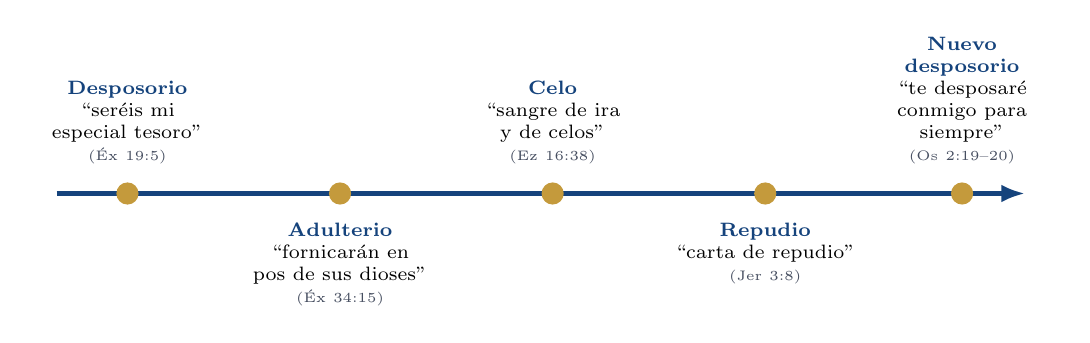
\begin{tikzpicture}[font=\scriptsize]
 \draw[line width=1.6pt,azul,-{Latex[length=3mm]}] (-0.3,0) -- (12.0,0);
 \foreach \x/\t/\b/\r/\pos in {0.6/{Desposorio}/{``seréis mi especial tesoro''}/{Éx 19:5}/above,
   3.3/{Adulterio}/{``fornicarán en pos de sus dioses''}/{Éx 34:15}/below,
   6.0/{Celo}/{``sangre de ira y de celos''}/{Ez 16:38}/above,
   8.7/{Repudio}/{``carta de repudio''}/{Jer 3:8}/below,
   11.2/{Nuevo desposorio}/{``te desposaré conmigo para siempre''}/{Os 2:19--20}/above}{
  \fill[dorado] (\x,0) circle (4pt);
  \node[\pos=7pt,text width=2.3cm,align=center] at (\x,0) {\textbf{\textcolor{azul}{\t}}\\ \b\\ {\tiny\color{gris}(\r)}};}
\end{tikzpicture}\par\medskip
\begin{columns}[t,onlytextwidth]
\begin{column}{0.49\textwidth}
\begin{cita}Y saciaré mi ira sobre ti, y se apartará de ti mi celo, y descansaré y no me enojaré más.\fuente{(Ez 16:42, RVR1960)}\end{cita}
\end{column}
\begin{column}{0.49\textwidth}\small
Los profetas leen la historia de Israel como un \destacar{matrimonio}. El celo es la reacción del Esposo fiel; su meta no es el divorcio sino un \destacar{nuevo desposorio} ``en justicia, juicio, benignidad y misericordia'' (Os 2:19).
\end{column}
\end{columns}
\end{frame}

% ------------------------------------------------------------------
\section{Manifestación}

\begin{frame}{¿Cómo se manifiesta?}
\begin{columns}[t,onlytextwidth]
\begin{column}{0.40\textwidth}\small
Se manifiesta como:
\begin{itemize}
\item disciplina;
\item juicio correctivo;
\item purificación;
\item defensa pública de su gloria;
\item guerra contra los ídolos.
\end{itemize}
\begin{tcolorbox}[colback=papiro,colframe=dorado,boxrule=1.2pt,arc=3pt]
\scriptsize No es exactamente ira general: es ira \destacar{dirigida contra la rivalidad idolátrica}.
\end{tcolorbox}
\end{column}
\begin{column}{0.58\textwidth}
\begin{cita}habló el rey y dijo: ¿No es ésta la gran Babilonia que yo edifiqué\ldots{} para gloria de mi majestad?\fuente{(Dn 4:30, RVR1960)}\end{cita}
\begin{cita}Al momento un ángel del Señor le hirió, por cuanto no dio la gloria a Dios; y expiró comido de gusanos.\fuente{(Hch 12:23, RVR1960)}\end{cita}
\scriptsize Nabucodonosor es humillado ``hasta que reconozcas que el Altísimo tiene el dominio'' (Dn 4:32) y termina alabando (4:37): disciplina que restaura. Herodes no: ``no dio la gloria a Dios''.
\end{column}
\end{columns}
\end{frame}

\begin{frame}{Fuego consumidor}
\begin{columns}[t,onlytextwidth]
\begin{column}{0.50\textwidth}
\begin{cita}Porque \SENOR{} tu Dios es fuego consumidor, Dios celoso.\fuente{(Dt 4:24, RVR1960)}\end{cita}
\begin{center}\heb{אֵשׁ אֹכְלָה הוּא אֵל קַנָּא}\end{center}
\begin{cita}Así que, recibiendo nosotros un reino inconmovible, tengamos gratitud, y mediante ella sirvamos a Dios agradándole con temor y reverencia; porque nuestro Dios es fuego consumidor.\fuente{(He 12:28--29, RVR1960)}\end{cita}
\end{column}
\begin{column}{0.48\textwidth}\small
Israel oyó a Dios ``de en medio del fuego'' y ``ninguna figura'' vio (Dt 4:12, 15). Por eso el fuego va unido a la prohibición: ``no os hagáis escultura o imagen'' (Dt 4:23). \destacar{El Dios sin figura no admite rival}.\par\medskip
Hebreos dirige la frase a la iglesia: el celo sostiene una adoración ``con temor y reverencia'', que ``se desarrolla mejor al recordar frecuentemente que `nuestro Dios es fuego consumidor'{}'' (Pink, 2020, cap. 18).\par\medskip
No se piensa desde nuestros celos: tampoco el amor de Dios es ``una especie de amable debilidad'' (Pink, 2020, cap. 16).
\end{column}
\end{columns}
\end{frame}

\begin{frame}{El celo que defiende a su pueblo}
\scriptsize\renewcommand{\arraystretch}{1.18}
\begin{tabular}{@{}>{\RaggedRight\arraybackslash}p{1.6cm}>{\RaggedRight\arraybackslash}p{6.4cm}>{\RaggedRight\arraybackslash}p{3.8cm}@{}}
\toprule
\textbf{Texto} & \textbf{RVR1960} & \textbf{Hebreo} \\ \midrule
Zac 1:14 & ``Celé con gran celo a Jerusalén y a Sion'' & \heb{קִנֵּאתִי לִירוּשָׁלִַם} \\
Zac 8:2 & ``Celé a Sion con gran celo, y con gran ira la celé'' & \heb{קִנְאָה גְדוֹלָה וְחֵמָה גְדוֹלָה} \\
Jl 2:18 & ``Y \SENOR, solícito por su tierra, perdonará a su pueblo'' & \heb{וַיְקַנֵּא יְהוָה לְאַרְצוֹ} \\
Ez 39:25 & ``tendré misericordia de toda la casa de Israel, y me mostraré celoso por mi santo nombre'' & \heb{וְקִנֵּאתִי לְשֵׁם קָדְשִׁי} \\
Is 59:17 & ``se cubrió de celo como de manto'' & \heb{וַיַּעַט כַּמְעִיל קִנְאָה} \\
\bottomrule
\end{tabular}\par\medskip
\small\RaggedRight El título de tu archivo lo dice: ``\destacar{celo por su pueblo}''. El mismo fuego que consume ídolos protege a Sion. En Ez 39:25 misericordia y celo están en la misma frase.\par\smallskip
\precision{en Jl 2:18 la RVR1960 traduce ``solícito''; el hebreo dice ``tuvo celo por su tierra'' (\emph{vayqanné}). La cita ``\SENOR{} se llenará de celo'' de tu material no es de la RVR1960.}
\end{frame}

% ------------------------------------------------------------------
\section{En Israel}

\begin{frame}{Baal-peor}
\centering
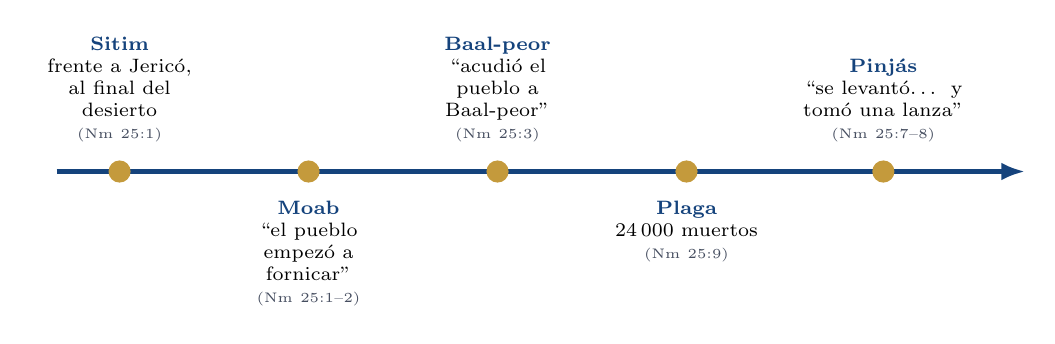
\begin{tikzpicture}[font=\scriptsize]
 \draw[line width=1.6pt,azul,-{Latex[length=3mm]}] (-0.3,0) -- (12.0,0);
 \foreach \x/\t/\b/\r/\pos in {0.5/{Sitim}/{frente a Jericó, al final del desierto}/{Nm 25:1}/above,
   2.9/{Moab}/{``el pueblo empezó a fornicar''}/{Nm 25:1--2}/below,
   5.3/{Baal-peor}/{``acudió el pueblo a Baal-peor''}/{Nm 25:3}/above,
   7.7/{Plaga}/{24\,000 muertos}/{Nm 25:9}/below,
   10.2/{Pinjás}/{``se levantó\ldots{} y tomó una lanza''}/{Nm 25:7--8}/above}{
  \fill[dorado] (\x,0) circle (4pt);
  \node[\pos=7pt,text width=2.1cm,align=center] at (\x,0) {\textbf{\textcolor{azul}{\t}}\\ \b\\ {\tiny\color{gris}(\r)}};}
\end{tikzpicture}\par\medskip
\begin{columns}[t,onlytextwidth]
\begin{column}{0.49\textwidth}
\begin{cita}Así acudió el pueblo a Baal-peor; y el furor de \SENOR{} se encendió contra Israel.\fuente{(Nm 25:3, RVR1960)}\end{cita}
\end{column}
\begin{column}{0.49\textwidth}\small
A las puertas de la tierra, Israel repite el pecado del Sinaí: inmoralidad y culto a otro dios. \heb{וַיִּצָּמֶד} (\emph{vayyitsámed}): ``se unció'', ``se ató'' a Baal, como un yugo.
\end{column}
\end{columns}
\end{frame}

\begin{frame}{Pinjás: celo compartido}
\fotolado{panel_numeros25.jpg}{Elaboración propia: Nm 25:11 en texto hebreo consonántico (BHS).}
\begin{columns}[c,onlytextwidth]
\begin{column}{0.58\textwidth}
\begin{cita}Finees hijo de Eleazar, hijo del sacerdote Aarón, ha hecho apartar mi furor de los hijos de Israel, llevado de celo entre ellos; por lo cual yo no he consumido en mi celo a los hijos de Israel. Por tanto diles: He aquí yo establezco mi pacto de paz con él; y tendrá él, y su descendencia después de él, el pacto del sacerdocio perpetuo, por cuanto tuvo celo por su Dios e hizo expiación por los hijos de Israel.\fuente{(Nm 25:11--13, RVR1960)}\end{cita}
\end{column}
\begin{column}{0.40\textwidth}\end{column}
\end{columns}
\end{frame}

\begin{frame}{Nm 25:11--13 en hebreo}
\begin{center}\heb{הֵשִׁיב אֶת־חֲמָתִי מֵעַל בְּנֵי־יִשְׂרָאֵל בְּקַנְאוֹ אֶת־קִנְאָתִי בְּתוֹכָם}\\[2pt]\heb{תַּחַת אֲשֶׁר קִנֵּא לֵאלֹהָיו וַיְכַפֵּר עַל־בְּנֵי יִשְׂרָאֵל}\end{center}
\scriptsize\renewcommand{\arraystretch}{1.13}
\begin{tabular}{@{}>{\RaggedRight\arraybackslash}p{3.1cm}>{\RaggedRight\arraybackslash}p{1.1cm}>{\RaggedRight\arraybackslash}p{7.6cm}@{}}
\toprule
\textbf{Término} & \textbf{Raíz} & \textbf{Sentido} \\ \midrule
\heb{הֵשִׁיב אֶת־חֲמָתִי} & \heb{שׁוב} & ``hizo volver mi furor'': lo apartó. \\
\heb{בְּקַנְאוֹ אֶת־קִנְאָתִי} & \heb{קנא} & ``al celar \destacar{mi} celo'': Pinjás no tuvo un celo propio, compartió el de Dios. La RVR1960: ``llevado de celo''. \\
\heb{בְּרִיתִי שָׁלוֹם} & \heb{שׁלם} & ``mi pacto de paz'': el celo termina en paz. \\
\heb{קִנֵּא לֵאלֹהָיו} & \heb{קנא} & ``tuvo celo \destacar{por} su Dios'' (con \heb{לְ}). \\
\heb{וַיְכַפֵּר} & \heb{כפר} & ``e hizo expiación'': cubrió el pecado del pueblo; la plaga se detuvo. \\
\bottomrule
\end{tabular}\par\medskip
\begin{cita}Entonces se levantó Finees e hizo juicio, Y se detuvo la plaga; Y le fue contado por justicia De generación en generación para siempre.\fuente{(Sal 106:30--31, RVR1960)}\end{cita}
\precision{``le fue contado por justicia'' (\heb{וַתֵּחָשֶׁב לוֹ לִצְדָקָה}) es casi la fórmula de Abraham en Gn 15:6, que Pablo cita en Ro 4:3.}
\end{frame}

\begin{frame}{Elías en Horeb}
\begin{columns}[t,onlytextwidth]
\begin{column}{0.52\textwidth}
\begin{cita}¿Qué haces aquí, Elías? El respondió: He sentido un vivo celo por \SENOR{} Dios de los ejércitos; porque los hijos de Israel han dejado tu pacto\ldots{} y sólo yo he quedado.\fuente{(1 R 19:9--10, RVR1960)}\end{cita}
\begin{center}\heb{קַנֹּא קִנֵּאתִי לַיהוָה אֱלֹהֵי צְבָאוֹת}\end{center}
\scriptsize \emph{qannó qinnetí}: infinitivo absoluto + verbo, ``celar, celé'': ``he celado ardientemente''.
\end{column}
\begin{column}{0.46\textwidth}\small
\begin{itemize}
\item Dios no está en el viento, ni en el terremoto, ni en el fuego, sino en \heb{קוֹל דְּמָמָה דַקָּה}, ``un silbo apacible y delicado'' (19:12).
\item Elías repite su queja dos veces (19:10, 14). Dios lo corrige: ``yo haré que queden en Israel \destacar{siete mil}'' (19:18).
\item El celo humano, aun por Dios, puede terminar en soledad y amargura. El de Dios guarda un \destacar{remanente}.
\end{itemize}
\end{column}
\end{columns}
\end{frame}

% ------------------------------------------------------------------
\section{Judaísmo}

\begin{frame}{La Mekhilta: dueño de su celo}
\begin{columns}[t,onlytextwidth]
\begin{column}{0.52\textwidth}\small
Sobre ``Dios celoso'' (Éx 20:5), la \emph{Mekhilta de Rabí Ismael} (Bajódesh 6) pregunta: ``¿Acaso soy un Dios de celo?'', y responde:
\begin{center}\heb{אֲנִי שַׁלִּיט בַּקִּנְאָה}\\ \heb{וְאֵין הַקִּנְאָה שׁוֹלֶטֶת בִּי}\end{center}
``Yo domino el celo, y el celo no me domina a mí''. Lo compara con el sueño: ``He aquí, no se adormecerá ni dormirá el que guarda a Israel'' (Sal 121:4).
\end{column}
\begin{column}{0.46\textwidth}\small
Otra explicación (ibíd.):
\begin{center}\heb{בְּקִנְאָה אֲנִי נִפְרָע מֵהֶם מִן עֲבוֹדָה זָרָה}\\ \heb{אֲבָל רַחוּם וְחַנּוּן אֲנִי בִּדְבָרִים אֲחֵרִים}\end{center}
``Con celo castigo la idolatría; pero en las demás cosas soy misericordioso y clemente''.\par\smallskip
\precision{interpretación rabínica; hebreo según la edición Beeri (Sefaria); traducción propia.}
\end{column}
\end{columns}\par\medskip
\small\RaggedRight Los sabios ven lo mismo que tu material: el celo de Dios \destacar{no es pasión descontrolada}; es soberano, y apunta específicamente a la idolatría.
\end{frame}

\begin{frame}{Rabán Gamaliel y los filósofos}
\begin{columns}[t,onlytextwidth]
\begin{column}{0.49\textwidth}\scriptsize
\textbf{El perro con el nombre del padre} (\emph{Avodá Zará} 54b): un filósofo pregunta por qué Dios, ``fuego consumidor, Dios celoso'' (Dt 4:24), se enoja con los idólatras y no con el ídolo. Gamaliel responde con una parábola: un hijo pone a su perro el nombre de su padre y jura ``por la vida del perro, mi padre''. ¿Con quién se enoja el rey? \destacar{Con el hijo}, no con el perro.\par\smallskip
\textbf{Con los vivos, no con los muertos} (ibíd.; \emph{Mekhilta}): un rey que sale a la guerra pelea con los vivos. El ídolo está muerto.
\end{column}
\begin{column}{0.49\textwidth}\scriptsize
\textbf{La segunda esposa} (\emph{Avodá Zará} 55a): Agripas pregunta: ``¿No se tiene celo solo de un igual? El sabio del sabio, el fuerte del fuerte, el rico del rico''. Gamaliel responde:
\begin{center}\heb{לְאָדָם שֶׁנָּשָׂא אִשָּׁה עַל אִשְׁתּוֹ}\end{center}
Si el hombre toma una segunda esposa \destacar{superior} a la primera, esta no tiene celos; si es \destacar{inferior}, sí los tiene.\par\smallskip
El celo de Dios no prueba que el ídolo sea rival a su altura; prueba que es \destacar{indigno}: ``lo que no es Dios'' (Dt 32:21).
\end{column}
\end{columns}\par\smallskip
\precision{lecturas rabínicas; Talmud de Babilonia, edición William Davidson (Sefaria).}
\end{frame}

\begin{frame}{Rashi, Ónkelos y Maimónides}
\scriptsize\renewcommand{\arraystretch}{1.18}
\begin{tabular}{@{}>{\RaggedRight\arraybackslash}p{2.3cm}>{\RaggedRight\arraybackslash}p{9.5cm}@{}}
\toprule
\textbf{Rashi} (Éx 20:5) & \heb{מְקַנֵּא לִפָּרַע וְאֵינוֹ עוֹבֵר עַל מִדָּתוֹ לִמְחֹל עַל עֲבוֹדַת אֱלִילִים}: ``Es celoso para castigar y no pasa por alto su medida para perdonar la idolatría''. Todo \emph{qanná} significa ``dar el corazón a castigar''. \\
\textbf{Rashi} (Éx 34:14) & \heb{אוֹחֵז בְּנִצְחוֹנוֹ וּפוֹרֵעַ מֵאוֹיְבָיו}: ``se aferra a su victoria y castiga a sus enemigos''. \\
\textbf{Ónkelos} (Dt 4:24) & \heb{מֵימְרֵיהּ אֶשָּׁא אָכְלָא הוּא אֵל קַנָּא}: ``\destacar{su Palabra} (\emph{Memrá}) es fuego consumidor, Dios celoso''. El Targum evita decir que Dios mismo es fuego. \\
\textbf{Maimónides} (\emph{Guía} I:36) & ``En toda la Torá y en los profetas no encontrarás `ira', `enojo' ni `\destacar{celo}' sino en relación con la idolatría''. Por eso llama ``enemigo'' de Dios solo al idólatra. \\
\bottomrule
\end{tabular}\par\medskip
\begin{columns}[t,onlytextwidth]
\begin{column}{0.55\textwidth}\small
Maimónides confirma la tesis de tu sermón con una lectura de toda la Biblia: el celo de Dios tiene \destacar{un solo blanco}, la idolatría.
\end{column}
\begin{column}{0.43\textwidth}
\precision{Maimónides añade que creer que Dios es corpóreo provoca su celo más que la idolatría misma (I:36). Lecturas judías medievales.}
\end{column}
\end{columns}
\end{frame}

\begin{frame}{Pinjás y Elías en la tradición}
\scriptsize\renewcommand{\arraystretch}{1.16}
\begin{tabular}{@{}>{\RaggedRight\arraybackslash}p{3.0cm}>{\RaggedRight\arraybackslash}p{8.8cm}@{}}
\toprule
\textbf{Misná} \emph{Sanedrín} 9:6 & \heb{קַנָּאִין פּוֹגְעִין בּוֹ}, ``los celosos lo hieren'': caso excepcional, limitado por la halajá; el Talmud lo rodea de condiciones (\emph{Sanedrín} 82a). \\
\textbf{Sifré} \emph{Bemidbar} 131 & Pinjás es ``celoso hijo de celoso'' (\heb{קַנָּאִי בֶּן קַנָּאִי}). Sobre ``tuvo celo por su Dios'' cita Is 53:12: ``por cuanto derramó su vida hasta la muerte''. Y lee ``e hizo expiación'' como algo que sigue haciendo hasta la resurrección de los muertos. \\
\textbf{Targum Pseudo-Jonatán} (Éx 6:18; Nm 25:12) & \heb{פִּינְחָס הוּא אֵלִיָּהוּ}: ``Pinjás es Elías'', que será enviado al final de los días; Dios lo hará ``ángel del pacto'' (cf. Mal 3:1). \\
\textbf{\emph{Pirqé de Rabí Eliézer}} 29 & a Elías, que dice ``he celado ardientemente'', Dios le responde: ``\destacar{siempre estás celando}''. \\
\textbf{1 Macabeos} 2:26, 54 & Matatías ``ardió de celo por la ley, como lo hizo Pinjás''; ``Pinjás, nuestro padre, por su ardiente celo recibió el pacto del sacerdocio eterno''. \\
\textbf{Qumrán} (1QS IX, 23) & el maestro de la comunidad debe ser ``hombre celoso por el precepto'', a la espera del día de la venganza. \\
\bottomrule
\end{tabular}\par\smallskip
\precision{interpretaciones judías antiguas. Rabínicos según Sefaria; 1 Macabeos según la LXX de Rahlfs-Hanhart (traducción propia); 1QS según García Martínez (1992): conviene cotejar en la Leon Levy Dead Sea Scrolls Digital Library.}
\end{frame}

% ------------------------------------------------------------------
\section{Isaías 9}

\begin{frame}{Contexto: Acaz y la crisis siria}
\centering
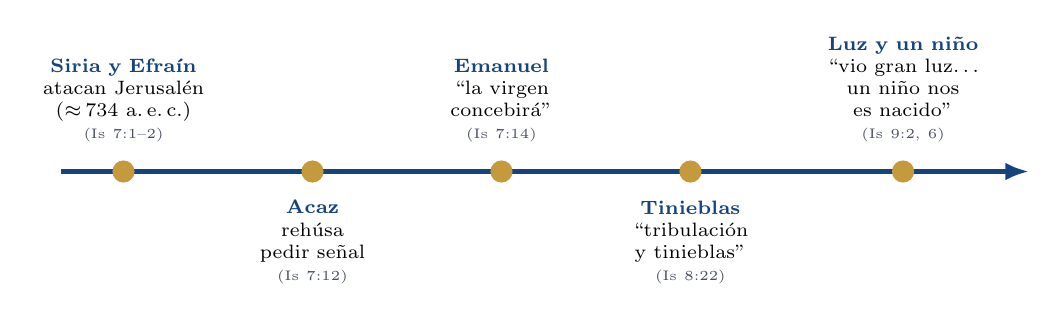
\begin{tikzpicture}[font=\scriptsize]
 \draw[line width=1.6pt,azul,-{Latex[length=3mm]}] (-0.3,0) -- (12.0,0);
 \foreach \x/\t/\b/\r/\pos in {0.5/{Siria y Efraín}/{atacan Jerusalén ($\approx$\,734 a.\,e.\,c.)}/{Is 7:1--2}/above,
   2.9/{Acaz}/{rehúsa pedir señal}/{Is 7:12}/below,
   5.3/{Emanuel}/{``la virgen concebirá''}/{Is 7:14}/above,
   7.7/{Tinieblas}/{``tribulación y tinieblas''}/{Is 8:22}/below,
   10.4/{Luz y un niño}/{``vio gran luz\ldots{} un niño nos es nacido''}/{Is 9:2, 6}/above}{
  \fill[dorado] (\x,0) circle (4pt);
  \node[\pos=7pt,text width=2.2cm,align=center] at (\x,0) {\textbf{\textcolor{azul}{\t}}\\ \b\\ {\tiny\color{gris}(\r)}};}
\end{tikzpicture}\par\medskip
\begin{columns}[t,onlytextwidth]
\begin{column}{0.49\textwidth}
\begin{cita}El pueblo que andaba en tinieblas vio gran luz; los que moraban en tierra de sombra de muerte, luz resplandeció sobre ellos.\fuente{(Is 9:2 [9:1], RVR1960)}\end{cita}
\end{column}
\begin{column}{0.49\textwidth}\small
El rey de David (\destacar{Acaz}) es infiel y busca la ayuda de Asiria (2 R 16:7). Humanamente, la promesa a David está en peligro. Justo ahí Isaías anuncia un hijo de David con un reino ``sin límite''.
\end{column}
\end{columns}
\end{frame}

\begin{frame}{Texto: Is 9:6--7 [9:5--6]}
\fotolado{panel_isaias9.jpg}{Elaboración propia: Is 9:7 [9:6] en texto hebreo consonántico (BHS), con la \emph{mem} cerrada de \emph{lemarbé}.}
\begin{columns}[c,onlytextwidth]
\begin{column}{0.58\textwidth}
\begin{cita}Porque un niño nos es nacido, hijo nos es dado, y el principado sobre su hombro; y se llamará su nombre Admirable, Consejero, Dios Fuerte, Padre Eterno, Príncipe de Paz. Lo dilatado de su imperio y la paz no tendrán límite, sobre el trono de David y sobre su reino, disponiéndolo y confirmándolo en juicio y en justicia desde ahora y para siempre. \destacar{El celo de \SENOR{} de los ejércitos hará esto.}\fuente{(Is 9:6--7 [9:5--6], RVR1960)}\end{cita}
\end{column}
\begin{column}{0.40\textwidth}\end{column}
\end{columns}
\end{frame}

\begin{frame}{Is 9:6--7 en hebreo}
\begin{center}\heb{כִּי־יֶלֶד יֻלַּד־לָנוּ בֵּן נִתַּן־לָנוּ וַתְּהִי הַמִּשְׂרָה עַל־שִׁכְמוֹ}\\[2pt]
\heb{וַיִּקְרָא שְׁמוֹ פֶּלֶא יוֹעֵץ אֵל גִּבּוֹר אֲבִיעַד שַׂר־שָׁלוֹם}\\[2pt]
\heb{לְםַרְבֵּה הַמִּשְׂרָה וּלְשָׁלוֹם אֵין־קֵץ עַל־כִּסֵּא דָוִד}\\[2pt]
\heb{קִנְאַת יְהוָה צְבָאוֹת תַּעֲשֶׂה־זֹּאת}\end{center}
\scriptsize\renewcommand{\arraystretch}{1.1}
\begin{tabular}{@{}>{\RaggedRight\arraybackslash}p{3.0cm}>{\RaggedRight\arraybackslash}p{8.8cm}@{}}
\toprule
\heb{יֶלֶד יֻלַּד}\newline \heb{בֵּן נִתַּן} & ``un niño nos ha nacido, un hijo nos ha sido dado'': nacido (humano) y \destacar{dado} (don de Dios). \\
\heb{אֵל גִּבּוֹר} \emph{El gibbor} & ``Dios Fuerte'': en Is 10:21 el mismo título es Dios mismo (``volverá al Dios fuerte''). \\
\heb{לְםַרְבֵּה} \emph{lemarbé} & ``para multiplicar'': el texto masorético escribe una \emph{mem} final (\heb{ם}) en medio de la palabra. \\
\heb{קִנְאַת יְהוָה צְבָאוֹת} & ``el celo del \SENOR{} de los ejércitos'': \emph{qin'at}, sustantivo en estado constructo. \\
\heb{תַּעֲשֶׂה־זֹּאת} \emph{ta'asé zot} & ``hará esto'': verbo \destacar{femenino}, concuerda con \emph{qin'á}. El celo mismo es el sujeto que actúa. \\
\bottomrule
\end{tabular}
\end{frame}

\begin{frame}{El celo como sujeto}
\scriptsize\renewcommand{\arraystretch}{1.2}
\begin{tabular}{@{}>{\RaggedRight\arraybackslash}p{2.4cm}>{\RaggedRight\arraybackslash}p{5.0cm}>{\RaggedRight\arraybackslash}p{4.4cm}@{}}
\toprule
\textbf{Testigo} & \textbf{Texto} & \textbf{Observación} \\ \midrule
TM (9:6) & \heb{קִנְאַת יְהוָה צְבָאוֹת תַּעֲשֶׂה־זֹּאת} & el celo es el agente \\
LXX (9:6) & \grc{ὁ ζῆλος κυρίου σαβαωθ ποιήσει ταῦτα} & ``el celo del Señor Sabaot hará esto'' \\
Targum Jonatán (9:6) & \heb{בְּמֵימְרָא דַייָ צְבָאוֹת תִּתְעֲבֵיד דָא} & ``por la \destacar{Palabra} del \SENOR{} de los ejércitos se hará esto'' \\
\bottomrule
\end{tabular}\par\medskip
\begin{columns}[t,onlytextwidth]
\begin{column}{0.52\textwidth}\small
\begin{itemize}
\item Isaías no dice ``el poder'' ni ``la sabiduría'' del \SENOR: dice su \destacar{celo}. La venida del rey prometido nace del amor ardiente de Dios por su pueblo y por su promesa.
\item ``De los ejércitos'': el mismo título con que Elías celó por Dios (1 R 19:10). Aquí es Dios quien cela.
\end{itemize}
\end{column}
\begin{column}{0.46\textwidth}
\precision{(textual) el Targum sustituye ``celo'' por \emph{Memrá}, ``Palabra'', como hace en otros lugares para evitar atribuir pasiones a Dios. La LXX conserva \grc{ζῆλος}.}
\end{column}
\end{columns}
\end{frame}

\begin{frame}{Tres veces la misma frase}
\centering
\begin{tikzpicture}[font=\scriptsize]
 \node[draw=dorado,line width=1.6pt,fill=azul,text=papiro,rounded corners=3pt,text width=4.6cm,align=center,inner sep=5pt] (f) at (0,0) {\heb{קִנְאַת יְהוָה צְבָאוֹת תַּעֲשֶׂה־זֹּאת}\\ ``El celo del \SENOR{} de los ejércitos hará esto''};
 \node[caja,text width=3.4cm,align=center] (a) at (-4.5,-2.1) {\textbf{Is 9:7 [9:6]}\\ el hijo de David y su reino sin fin};
 \node[caja,text width=3.4cm,align=center] (b) at (0,-2.1) {\textbf{Is 37:32}\\ ``de Jerusalén saldrá un remanente'' (Ezequías ante Senaquerib)};
 \node[caja,text width=3.4cm,align=center] (c) at (4.5,-2.1) {\textbf{2 R 19:31}\\ el mismo oráculo en Reyes};
 \foreach \i in {a,b,c}\draw[-{Latex[length=2.5mm]},dorado,line width=1.1pt](f)--(\i);
\end{tikzpicture}\par\medskip
\begin{columns}[t,onlytextwidth]
\begin{column}{0.52\textwidth}
\begin{cita}Porque yo ampararé a esta ciudad para salvarla, por amor de mí mismo, y por amor de David mi siervo.\fuente{(Is 37:35, RVR1960)}\end{cita}
\end{column}
\begin{column}{0.46\textwidth}\small
El celo salva a Jerusalén ``por amor de mí mismo, y por amor de \destacar{David}''. El mismo celo que preserva un remanente traerá al Hijo de David.
\end{column}
\end{columns}
\precision{(textual) en 2 R 19:31 el códice escribe ``el celo del \SENOR'' y los masoretas leen ``de los ejércitos'' (\emph{qeré} sin \emph{ketiv}). La conexión entre los tres textos es lectura propia.}
\end{frame}

\begin{frame}{La \emph{mem} cerrada}
\begin{columns}[t,onlytextwidth]
\begin{column}{0.52\textwidth}\small
\textbf{Talmud} (\emph{Sanedrín} 94a): ``¿Por qué toda \emph{mem} en medio de palabra es abierta, y esta es cerrada?''
\begin{center}\heb{בִּיקֵּשׁ הַקָּדוֹשׁ בָּרוּךְ הוּא לַעֲשׂוֹת}\\ \heb{חִזְקִיָּהוּ מָשִׁיחַ וְסַנְחֵרִיב גּוֹג וּמָגוֹג}\end{center}
``El Santo, bendito sea, quiso hacer a Ezequías Mesías y a Senaquerib Gog y Magog''. La medida de la justicia objetó: Ezequías no cantó alabanza después de su liberación. ``Por eso se cerró''.
\end{column}
\begin{column}{0.46\textwidth}\small
\textbf{Rashi} (a Is 9:6): ``el celo del \SENOR{} de los ejércitos'', que tuvo celo por Sion contra Aram y Pecaj; ``hará esto'',
\begin{center}\heb{וְלֹא אָחָז רָאוּי לְכָךְ}\\ \heb{וְאַף זְכוּת אָבוֹת תַּמָּה}\end{center}
``y Acaz no es digno de ello, y aun el mérito de los padres se ha agotado''.\par\smallskip
\destacar{El celo de Dios actúa donde no hay mérito}: es pura gracia.
\end{column}
\end{columns}\par\smallskip
\precision{interpretaciones rabínicas (Sefaria, edición William Davidson y edición vocalizada de Rashi). La \emph{mem} cerrada es un dato del texto masorético; su sentido es lectura de los sabios.}
\end{frame}

\begin{frame}{¿Quién es el niño?}
\scriptsize\renewcommand{\arraystretch}{1.2}
\begin{tabular}{@{}>{\RaggedRight\arraybackslash}p{2.6cm}>{\RaggedRight\arraybackslash}p{5.2cm}>{\RaggedRight\arraybackslash}p{4.0cm}@{}}
\toprule
\textbf{Lectura} & \textbf{Texto} & \textbf{Observación} \\ \midrule
Targum Jonatán (9:5) & \heb{מְשִׁיחָא דִשְׁלָמָא יַסְגֵי עֲלָנָא בְּיוֹמוֹהִי}: ``el \destacar{Mesías}, en cuyos días abundará la paz sobre nosotros'' & la tradición judía antigua lee un texto mesiánico \\
Rashi (9:5) & Ezequías, hijo de Acaz; Dios lo llama ``Príncipe de paz'' & lectura histórica medieval \\
Lucas 1:32--33 & ``el Señor Dios le dará el trono de David su padre\ldots{} y su reino no tendrá fin'' & eco de Is 9:7 \\
Mateo 4:15--16 & cita Is 9:1--2: ``El pueblo asentado en tinieblas vio gran luz'' & Galilea, inicio del ministerio de Jesús \\
\bottomrule
\end{tabular}\par\medskip
\begin{columns}[t,onlytextwidth]
\begin{column}{0.55\textwidth}\small
Los nombres del niño superan a cualquier rey de Judá: ``Dios Fuerte'' (cf. Is 10:21), ``Padre Eterno'', un reino ``desde ahora y para siempre''. El Targum ya lo leía como el Mesías.
\end{column}
\begin{column}{0.43\textwidth}
\precision{la identificación con Jesús es la lectura del NT; Rashi la discute expresamente (lectura polémica medieval).}
\end{column}
\end{columns}
\end{frame}

\begin{frame}{Por qué el celo envía al Mesías}
\centering
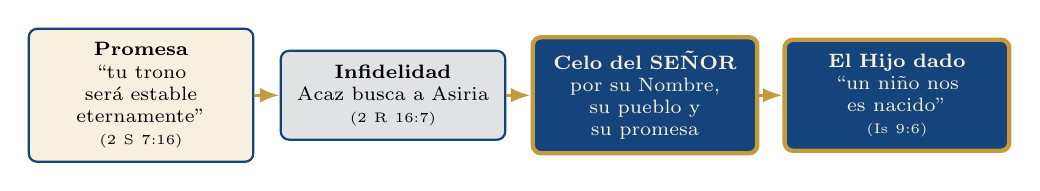
\begin{tikzpicture}[font=\scriptsize]
 \node[caja,text width=2.5cm,align=center] (a) at (0,0) {\textbf{Promesa}\\ ``tu trono será estable eternamente''\\ {\tiny(2 S 7:16)}};
 \node[caja,text width=2.5cm,align=center,fill=gris!18] (b) at (3.2,0) {\textbf{Infidelidad}\\ Acaz busca a Asiria\\ {\tiny(2 R 16:7)}};
 \node[draw=dorado,line width=1.6pt,fill=azul,text=papiro,rounded corners=3pt,text width=2.5cm,align=center,inner sep=5pt] (c) at (6.4,0) {\textbf{Celo del \SENOR}\\ por su Nombre, su pueblo y su promesa};
 \node[draw=dorado,line width=1.6pt,fill=azul,text=papiro,rounded corners=3pt,text width=2.5cm,align=center,inner sep=5pt] (d) at (9.6,0) {\textbf{El Hijo dado}\\ ``un niño nos es nacido''\\ {\tiny(Is 9:6)}};
 \draw[-{Latex[length=2.5mm]},dorado,line width=1.2pt] (a)--(b); \draw[-{Latex[length=2.5mm]},dorado,line width=1.2pt] (b)--(c); \draw[-{Latex[length=2.5mm]},dorado,line width=1.2pt] (c)--(d);
\end{tikzpicture}\par\medskip
\begin{columns}[t,onlytextwidth]
\begin{column}{0.52\textwidth}\small
\begin{itemize}
\item El celo es el amor de Dios que \destacar{no suelta} lo que es suyo (Cnt 8:6).
\item Por eso no solo destruye ídolos: también \destacar{rescata}. Frente a un rey infiel y un pueblo en tinieblas, Dios no abandona su promesa: envía al Rey.
\item En Is 9 el celo no es fuego contra Israel, sino ardor \destacar{a favor} de Israel.
\end{itemize}
\end{column}
\begin{column}{0.46\textwidth}
\begin{tcolorbox}[colback=papiro,colframe=dorado,boxrule=1.2pt,arc=3pt]
\small El Mesías no viene porque Israel lo mereciera, sino porque \destacar{Dios es celoso}: no permitirá que otro rey, otro dios u otra potencia se quede con su pueblo.
\end{tcolorbox}
\precision{síntesis teológica de esta serie.}
\end{column}
\end{columns}
\end{frame}

% ------------------------------------------------------------------
\section{En Cristo}

\begin{frame}{``El celo de tu casa me consume''}
\begin{columns}[t,onlytextwidth]
\begin{column}{0.50\textwidth}
\begin{cita}Y haciendo un azote de cuerdas, echó fuera del templo a todos\ldots{} y dijo a los que vendían palomas: Quitad de aquí esto, y no hagáis de la casa de mi Padre casa de mercado. Entonces se acordaron sus discípulos que está escrito: El celo de tu casa me consume.\fuente{(Jn 2:15--17, RVR1960)}\end{cita}
\end{column}
\begin{column}{0.48\textwidth}
\begin{center}\heb{כִּי־קִנְאַת בֵּיתְךָ אֲכָלָתְנִי}\\ \footnotesize (Sal 69:9 [69:10])\end{center}
\scriptsize\renewcommand{\arraystretch}{1.15}
\begin{tabular}{@{}>{\RaggedRight\arraybackslash}p{1.6cm}>{\RaggedRight\arraybackslash}p{4.0cm}@{}}
\toprule
Sal 69:9a & ``me consumió el celo de tu casa'' $\rightarrow$ \textbf{Juan 2:17} \\
Sal 69:9b & ``los denuestos de los que te vituperaban cayeron sobre mí'' $\rightarrow$ \textbf{Pablo, Ro 15:3} \\
\bottomrule
\end{tabular}\par\smallskip
\small Juan cita la primera mitad del verso; Pablo, la segunda. Cristo arde de celo por la casa de Dios y carga el oprobio de los que ofenden a Dios.
\end{column}
\end{columns}\par\smallskip
\precision{Juan cambia el pasado del Salmo (\grc{κατέφαγεν}) por futuro (\grc{καταφάγεταί}): ``me consumirá'', anticipo de la cruz (Carson, 1991).}
\end{frame}

\begin{frame}{``Os celo con celo de Dios''}
\fotolado{panel_2corintios11.jpg}{Elaboración propia: 2 Co 11:2 en escritura uncial (texto NA28), con \emph{nomina sacra}.}
\begin{columns}[c,onlytextwidth]
\begin{column}{0.58\textwidth}
\begin{cita}Porque os celo con celo de Dios; pues os he desposado con un solo esposo, para presentaros como una virgen pura a Cristo. Pero temo que como la serpiente con su astucia engañó a Eva, vuestros sentidos sean de alguna manera extraviados de la sincera fidelidad a Cristo.\fuente{(2 Co 11:2--3, RVR1960)}\end{cita}
\scriptsize\grc{ζηλῶ γὰρ ὑμᾶς θεοῦ ζήλῳ}: ``os celo con \destacar{celo de Dios}''. \grc{ἡρμοσάμην}: ``os comprometí en matrimonio''. Pablo actúa como el amigo del novio; el Esposo es Cristo, el papel que los profetas daban al \SENOR{} (Is 54:5; Os 2:19--20).
\end{column}
\begin{column}{0.40\textwidth}\end{column}
\end{columns}
\end{frame}

\begin{frame}{Provocar a celos: Dt 32 en Romanos}
\scriptsize\renewcommand{\arraystretch}{1.15}
\begin{tabular}{@{}>{\RaggedRight\arraybackslash}p{1.3cm}>{\RaggedRight\arraybackslash}p{5.3cm}>{\RaggedRight\arraybackslash}p{5.2cm}@{}}
\toprule
\textbf{Texto} & \textbf{Original} & \textbf{RVR1960} \\ \midrule
Dt 32:21 TM & \heb{הֵם קִנְאוּנִי בְלֹא־אֵל}\newline \heb{וַאֲנִי אַקְנִיאֵם בְּלֹא־עָם} & ``me movieron a celos con lo que no es Dios\ldots{} yo también los moveré a celos con un pueblo que no es pueblo'' \\
Dt 32:21 LXX & \grc{παρεζήλωσάν με ἐπ’ οὐ θεῷ\ldots{} κἀγὼ παραζηλώσω αὐτοὺς ἐπ’ οὐκ ἔθνει} & --- \\
Ro 10:19 & \grc{ἐγὼ παραζηλώσω ὑμᾶς ἐπ’ οὐκ ἔθνει} & ``Yo os provocaré a celos con un pueblo que no es pueblo'' \\
\bottomrule
\end{tabular}\par\medskip
\centering
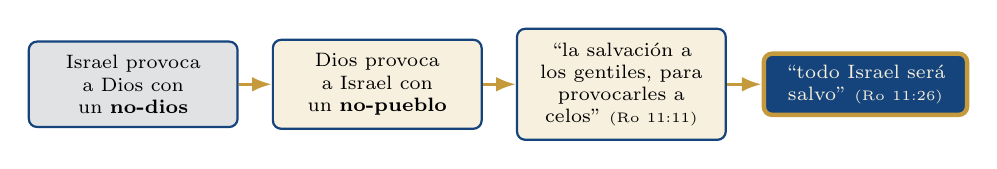
\begin{tikzpicture}[font=\scriptsize]
 \node[caja,text width=2.3cm,align=center,fill=gris!18] (a) at (0,0) {Israel provoca a Dios con un \textbf{no-dios}};
 \node[caja,text width=2.3cm,align=center] (b) at (3.1,0) {Dios provoca a Israel con un \textbf{no-pueblo}};
 \node[caja,text width=2.3cm,align=center] (c) at (6.2,0) {``la salvación a los gentiles, para provocarles a celos'' {\tiny(Ro 11:11)}};
 \node[draw=dorado,line width=1.6pt,fill=azul,text=papiro,rounded corners=3pt,text width=2.3cm,align=center,inner sep=4pt] (d) at (9.3,0) {``todo Israel será salvo'' {\tiny(Ro 11:26)}};
 \draw[-{Latex[length=2.5mm]},dorado,line width=1.1pt](a)--(b); \draw[-{Latex[length=2.5mm]},dorado,line width=1.1pt](b)--(c); \draw[-{Latex[length=2.5mm]},dorado,line width=1.1pt](c)--(d);
\end{tikzpicture}\par\smallskip
\small\RaggedRight Pablo descubre en el cántico de Moisés el \destacar{plan} del celo divino: Dios usa la misericordia hacia las naciones para despertar a Israel (Ro 11:14). El celo no termina en descarte: termina en salvación.
\end{frame}

\begin{frame}{``¿Provocaremos a celos al Señor?''}
\begin{columns}[t,onlytextwidth]
\begin{column}{0.50\textwidth}
\begin{cita}Por tanto, amados míos, huid de la idolatría\ldots{} lo que los gentiles sacrifican, a los demonios lo sacrifican, y no a Dios\ldots{} No podéis beber la copa del Señor, y la copa de los demonios\ldots{} ¿O provocaremos a celos al Señor? ¿Somos más fuertes que él?\fuente{(1 Co 10:14, 20--22, RVR1960)}\end{cita}
\end{column}
\begin{column}{0.48\textwidth}\small
\begin{itemize}
\item ``A los demonios\ldots{} y no a Dios'' cita Dt 32:17 (LXX \grc{ἔθυσαν δαιμονίοις καὶ οὐ θεῷ}).
\item ``¿Provocaremos a celos?'' (\grc{παραζηλοῦμεν}) es Dt 32:21.
\item El ``Señor'' es el de ``la copa del Señor'' y ``la mesa del Señor'': \destacar{Jesucristo}.
\item Pablo pone a Cristo en el lugar del Dios celoso del cántico de Moisés.
\end{itemize}
\precision{lectura cristológica sostenida por Fee (1987) y Hays (1989); es la lectura más probable por el contexto de la Cena.}
\end{column}
\end{columns}
\end{frame}

\begin{frame}{El celo de Saulo}
\begin{columns}[t,onlytextwidth]
\begin{column}{0.50\textwidth}
\begin{cita}y en el judaísmo aventajaba a muchos de mis contemporáneos en mi nación, siendo mucho más celoso de las tradiciones de mis padres.\fuente{(Gá 1:14, RVR1960)}\end{cita}
\begin{cita}en cuanto a celo, perseguidor de la iglesia\ldots{} Pero cuantas cosas eran para mí ganancia, las he estimado como pérdida por amor de Cristo.\fuente{(Flp 3:6--7, RVR1960)}\end{cita}
\end{column}
\begin{column}{0.48\textwidth}\small
\begin{itemize}
\item Pablo se describe como \grc{ζηλωτής} (Gá 1:14; Hch 22:3): en la línea de Pinjás, Elías y los Macabeos.
\item Ese celo lo llevó a \destacar{perseguir} a la iglesia.
\item De Israel dirá: ``tienen celo de Dios, pero no conforme a ciencia'' (Ro 10:2, \grc{οὐ κατ’ ἐπίγνωσιν}).
\item En Cristo, el celo no desaparece: cambia de \destacar{objeto} (2 Co 11:2).
\end{itemize}
\precision{el trasfondo de Pinjás en el ``celo'' de Pablo es tesis de Hengel (1989) y Wright (2013); Dunn (1998) la recoge.}
\end{column}
\end{columns}
\end{frame}

\begin{frame}{Un pueblo celoso de buenas obras}
\begin{columns}[c,onlytextwidth]
\begin{column}{0.52\textwidth}
\begin{cita}quien se dio a sí mismo por nosotros para redimirnos de toda iniquidad y purificar para sí un pueblo propio, celoso de buenas obras.\fuente{(Tit 2:14, RVR1960)}\end{cita}
\scriptsize\grc{λαὸν περιούσιον, ζηλωτὴν καλῶν ἔργων}: ``pueblo de su propiedad'' es la expresión de la LXX para la \emph{segul.lá} de Éx 19:5.
\end{column}
\begin{column}{0.46\textwidth}
\centering
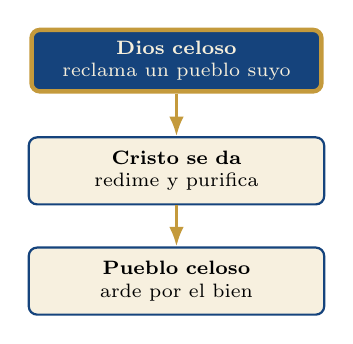
\begin{tikzpicture}[font=\scriptsize]
 \node[draw=dorado,line width=1.6pt,fill=azul,text=papiro,rounded corners=3pt,text width=3.4cm,align=center,inner sep=4pt] (a) at (0,1.4) {\textbf{Dios celoso}\\ reclama un pueblo suyo};
 \node[caja,text width=3.4cm,align=center] (b) at (0,0) {\textbf{Cristo se da}\\ redime y purifica};
 \node[caja,text width=3.4cm,align=center] (c) at (0,-1.4) {\textbf{Pueblo celoso}\\ arde por el bien};
 \draw[-{Latex[length=2.5mm]},dorado,line width=1.1pt](a)--(b); \draw[-{Latex[length=2.5mm]},dorado,line width=1.1pt](b)--(c);
\end{tikzpicture}
\end{column}
\end{columns}\par\smallskip
\precision{la autoría paulina de Tito se discute; la idea tiene respaldo en cartas indiscutidas (Gá 4:18: ``bueno es mostrar celo en lo bueno siempre'').}
\end{frame}

\begin{frame}{El celo de Dios, cumplido en Cristo}
\centering
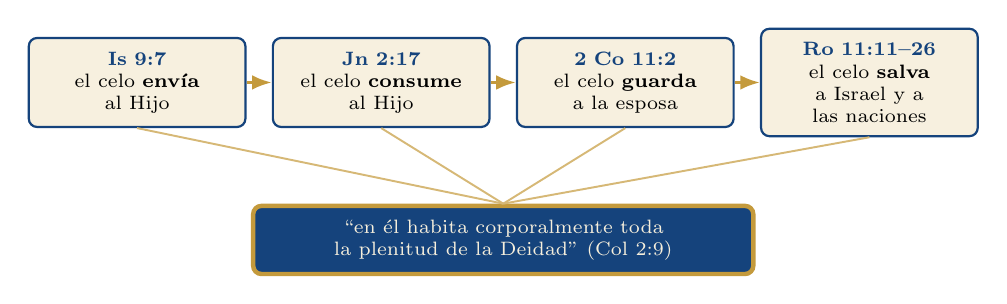
\begin{tikzpicture}[font=\scriptsize]
 \foreach \x/\y/\n/\t/\d in {0/0/a/{Is 9:7}/{el celo \textbf{envía} al Hijo},
   3.1/0/b/{Jn 2:17}/{el celo \textbf{consume} al Hijo},
   6.2/0/c/{2 Co 11:2}/{el celo \textbf{guarda} a la esposa},
   9.3/0/d/{Ro 11:11--26}/{el celo \textbf{salva} a Israel y a las naciones}}{
  \node[caja,text width=2.4cm,align=center] (\n) at (\x,\y) {\textbf{\textcolor{azul}{\t}}\\ \d};}
 \draw[-{Latex[length=2.5mm]},dorado,line width=1.1pt](a)--(b); \draw[-{Latex[length=2.5mm]},dorado,line width=1.1pt](b)--(c); \draw[-{Latex[length=2.5mm]},dorado,line width=1.1pt](c)--(d);
 \node[draw=dorado,line width=1.6pt,fill=azul,text=papiro,rounded corners=3pt,text width=6.0cm,align=center,inner sep=5pt] (e) at (4.65,-2.0) {``en él habita corporalmente toda la plenitud de la Deidad'' (Col 2:9)};
 \foreach \i in {a,b,c,d}\draw[dorado!70,line width=0.7pt](\i.south)--(e.north);
\end{tikzpicture}\par\medskip
\small\RaggedRight Pablo, judío formado en las Escrituras, lee el celo del Sinaí \destacar{cumplido en Cristo}: el Dios que no comparte su gloria la muestra ``en la faz de Jesucristo'' (2 Co 4:6). Quien ve el celo de Cristo por la casa de su Padre ve el celo del \SENOR.
\end{frame}

% ------------------------------------------------------------------
\section{Vivirlo}

\begin{frame}{¿Cómo me bendice?}
\begin{columns}[t,onlytextwidth]
\begin{column}{0.44\textwidth}\small
El celo de Dios me bendice porque:
\begin{itemize}
\item me rescata de mis ídolos;
\item me protege de la autodestrucción;
\item preserva el pacto;
\item me disciplina para restaurarme;
\item garantiza mi salvación.
\end{itemize}
\begin{center}\destacar{Sin el celo de Dios, pereceríamos.}\end{center}
\end{column}
\begin{column}{0.54\textwidth}
\begin{cita}Porque yo \SENOR, Dios tuyo, el Santo de Israel, soy tu Salvador; a Egipto he dado por tu rescate, a Etiopía y a Seba por ti. Porque a mis ojos fuiste de gran estima, fuiste honorable, y yo te amé.\fuente{(Is 43:3--4, RVR1960)}\end{cita}
\begin{cita}Y \SENOR, solícito por su tierra, perdonará a su pueblo. Responderá \SENOR, y dirá a su pueblo: He aquí yo os envío pan, mosto y aceite.\fuente{(Jl 2:18--19, RVR1960)}\end{cita}
\end{column}
\end{columns}
\end{frame}

\begin{frame}{Destruye mis ídolos antes que me destruyan}
\begin{columns}[t,onlytextwidth]
\begin{column}{0.50\textwidth}
\begin{cita}¡Oh almas adúlteras! ¿No sabéis que la amistad del mundo es enemistad contra Dios?\ldots{} ¿O pensáis que la Escritura dice en vano: El Espíritu que él ha hecho morar en nosotros nos anhela celosamente?\fuente{(Stg 4:4--5, RVR1960)}\end{cita}
\begin{cita}Yo reprendo y castigo a todos los que amo; sé, pues, celoso, y arrepiéntete.\fuente{(Ap 3:19, RVR1960)}\end{cita}
\end{column}
\begin{column}{0.48\textwidth}\small
\begin{itemize}
\item Santiago usa el lenguaje de Oseas: ``almas \destacar{adúlteras}''.
\item El ídolo promete vida y entrega muerte: ``lo que no es Dios'' no puede salvar.
\item La disciplina es \destacar{amor}: ``reprendo y castigo a todos los que amo''. El que ama, cela.
\item ``Hijitos, guardaos de los ídolos'' (1 Jn 5:21).
\end{itemize}
\end{column}
\end{columns}
\end{frame}

\begin{frame}{Un celo que se refleja}
\scriptsize\renewcommand{\arraystretch}{1.2}
\begin{tabular}{@{}>{\RaggedRight\arraybackslash}p{5.8cm}>{\RaggedRight\arraybackslash}p{6.0cm}@{}}
\toprule
\textbf{Celo conforme a Dios} & \textbf{Celo desviado} \\ \midrule
``tuvo celo por su Dios'': comparte el celo de Dios (Nm 25:11--13) & ``celo de Dios, pero no conforme a ciencia'' (Ro 10:2) \\
``Bueno es mostrar celo en lo bueno siempre'' (Gá 4:18) & ``Tienen celo por vosotros, pero no para bien'' (Gá 4:17) \\
``celoso de buenas obras'' (Tit 2:14) & ``celos amargos y contención'' (Stg 3:14--16); ``celos'' entre las obras de la carne (Gá 5:20) \\
``os celo con celo de Dios'' (2 Co 11:2) & ``en cuanto a celo, perseguidor de la iglesia'' (Flp 3:6) \\
``fervientes en espíritu, sirviendo al Señor'' (Ro 12:11) & ``sólo yo he quedado'' (1 R 19:10): celo que termina en soledad \\
\bottomrule
\end{tabular}\par\medskip
\small\RaggedRight El celo es comunicable \destacar{como reflejo}: el creyente arde por la gloria de Dios y por la pureza de la iglesia. Pero el celo humano necesita ``ciencia'', mansedumbre y la corrección que Dios dio a Elías.
\end{frame}

\begin{frame}{Cuatro respuestas al Dios celoso}
\centering
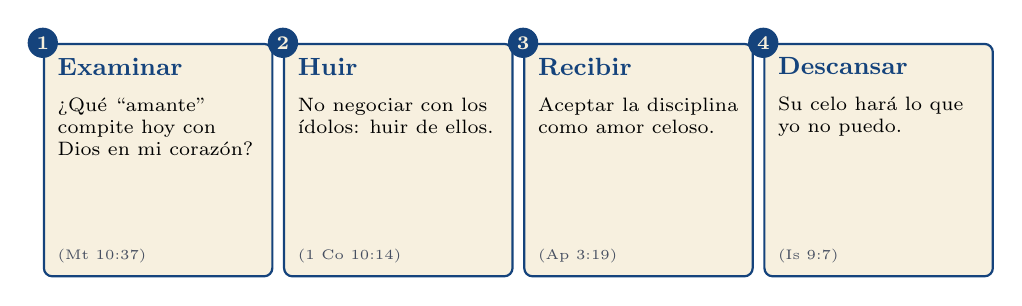
\begin{tikzpicture}
 \foreach \x/\n/\t/\d/\r in {0/1/{Examinar}/{¿Qué ``amante'' compite hoy con Dios en mi corazón?}/{Mt 10:37},
   3.05/2/{Huir}/{No negociar con los ídolos: huir de ellos.}/{1 Co 10:14},
   6.1/3/{Recibir}/{Aceptar la disciplina como amor celoso.}/{Ap 3:19},
   9.15/4/{Descansar}/{Su celo hará lo que yo no puedo.}/{Is 9:7}}{
  \node[caja,anchor=north] (b\n) at (\x,0) {\parbox[t][2.6cm][t]{2.55cm}{\RaggedRight
    {\small\textbf{\textcolor{azul}{\t}}}\\[5pt]\scriptsize \d\par\vfill{\tiny\color{gris}(\r)}}};
  \node[circle,fill=azul,text=papiro,font=\scriptsize\bfseries,inner sep=1.6pt] at (b\n.north west) {\n};}
\end{tikzpicture}\par\medskip
\small\RaggedRight ``El celo del \SENOR{} de los ejércitos hará esto'': la última palabra no la tiene mi fidelidad, sino su celo.
\end{frame}

% ------------------------------------------------------------------
\section{Síntesis}

\begin{frame}{Síntesis}
\begin{tcolorbox}[colback=papiro,colframe=azul,boxrule=1pt,arc=3pt]
\small ``\SENOR, cuyo nombre es Celoso, Dios celoso es'' (Éx 34:14). El celo de Dios es el \destacar{ardor} de su santo amor de pacto: no tolera rivales porque el rival es ``lo que no es Dios'' y destruye a su pueblo. Se enciende con la idolatría, se manifiesta en disciplina y juicio, y arde \destacar{por} Sion, por su Nombre y por su promesa. Por ese celo vino el Hijo de David (Is 9:7), ardió por la casa de su Padre (Jn 2:17), guarda a la iglesia como esposa (2 Co 11:2) y salvará a Israel y a las naciones (Ro 11:11--26).
\end{tcolorbox}
\scriptsize\renewcommand{\arraystretch}{1.15}
\begin{tabular}{@{}>{\RaggedRight\arraybackslash}p{2.4cm}>{\RaggedRight\arraybackslash}p{9.4cm}@{}}
\toprule
\textbf{Mirada} & \textbf{Aporte} \\ \midrule
Hebrea & \emph{qanná} como nombre y como adjetivo (Éx 34:14); solo de Dios; ardor; pacto como matrimonio; Pinjás y Elías; Is 9:7. \\
Judía & ``domino el celo'' (Mekhilta); solo contra la idolatría (Maimónides); la segunda esposa (AZ 55a); la \emph{mem} cerrada (Sanedrín 94a). \\
Teológica & ``fuego consumidor'' (Dt 4:24; He 12:29): el Dios sin figura no admite rival; reverencia, no celos humanos. \\
Paulina & ``celo de Dios'' por la iglesia; Dt 32:21 en Ro 10--11 y 1 Co 10:22; el celo de Saulo transformado; un pueblo celoso de buenas obras. \\
\bottomrule
\end{tabular}
\end{frame}

\begin{frame}{Para la reflexión}
\begin{cita}Mas alábese en esto el que se hubiere de alabar: en entenderme y conocerme, que yo soy \SENOR, que hago misericordia, juicio y justicia en la tierra; porque estas cosas quiero, dice \SENOR.\fuente{(Jer 9:24 [9:23], RVR1960)}\end{cita}
\begin{center}\heb{כִּי אֲנִי יְהוָה עֹשֶׂה חֶסֶד מִשְׁפָּט וּצְדָקָה בָּאָרֶץ}\end{center}
\small
\begin{itemize}
\item ¿Me molesta que Dios sea celoso, o me consuela saber que no me comparte con nadie?
\item ¿Qué ``no-dios'' (Dt 32:21) he puesto a competir con él?
\item Mi celo religioso, ¿se parece al de Pinjás, al de Elías en la cueva o al de Saulo antes de Damasco?
\item ¿Descanso en que ``el celo del \SENOR{} de los ejércitos hará esto''?
\end{itemize}
\end{frame}

% ------------------------------------------------------------------
\section{Glosario}

\begin{frame}{Glosario (1)}
\scriptsize
\begin{columns}[t,onlytextwidth]
\begin{column}{0.49\textwidth}
\begin{description}\setlength{\itemsep}{1pt}
\item[\emph{El gibbor}] (\heb{אֵל גִּבּוֹר}) ``Dios Fuerte'' (Is 9:6; 10:21).
\item[\emph{El qanná}] (\heb{אֵל קַנָּא}) ``Dios celoso'' (Éx 20:5; 34:14; Dt 4:24).
\item[\emph{Hiqní}] (\heb{הִקְנִיא}) provocar a celos (Dt 32:16, 21).
\item[\emph{Jemá}] (\heb{חֵמָה}) calor, furor; par de \emph{qin'á}.
\item[\emph{Kanná'im}] (\heb{קַנָּאִים}) ``celosos'', zelotes (Misná \emph{Sanedrín} 9:6).
\item[\emph{Memrá}] (\heb{מֵימְרָא}) ``Palabra'' del \SENOR{} en los targumes.
\item[\emph{Parazēlóō}] (\grc{παραζηλόω}) provocar a celos (Ro 10:19; 11:11, 14; 1 Co 10:22).
\item[\emph{Qanná}] (\heb{קַנָּא}) celoso; adjetivo solo de Dios.
\item[\emph{Qannó}] (\heb{קַנּוֹא}) celoso (Jos 24:19; Nah 1:2).
\end{description}
\end{column}
\begin{column}{0.49\textwidth}
\begin{description}\setlength{\itemsep}{1pt}
\item[\emph{Qinné}] (\heb{קִנֵּא}) tener celo por (\heb{לְ}); envidiar (\heb{בְּ}).
\item[\emph{Qin'á}] (\heb{קִנְאָה}) celo, ardor; celos; envidia.
\item[\emph{Qin'at YHWH tseva'ot}] (\heb{קִנְאַת יְהוָה צְבָאוֹת}) ``el celo del \SENOR{} de los ejércitos'' (Is 9:7; 37:32).
\item[\emph{Segul.lá}] (\heb{סְגֻלָּה}) tesoro personal (Éx 19:5).
\item[\emph{Sémel haqqin'á}] (\heb{סֵמֶל הַקִּנְאָה}) ``imagen del celo'' (Ez 8:3, 5).
\item[\emph{Shalhévetyá}] (\heb{שַׁלְהֶבֶתְיָה}) ``llama de Yah'' (Cnt 8:6).
\item[\emph{Zaná}] (\heb{זָנָה}) fornicar; ser infiel al pacto (Éx 34:15).
\item[\emph{Zēlos}] (\grc{ζῆλος}) celo, ardor; de \grc{ζέω}, hervir.
\item[\emph{Zēlōtēs}] (\grc{ζηλωτής}) celoso; zelote (Gá 1:14; Tit 2:14).
\end{description}
\end{column}
\end{columns}
\end{frame}

% ------------------------------------------------------------------
\section{Referencias}

\begin{frame}{Referencias}
\fontsize{5.4}{6.4}\selectfont
\begin{columns}[t,onlytextwidth]
\begin{column}{0.49\textwidth}
\refapa{Bauer, W., Danker, F.~W., Arndt, W.~F., \& Gingrich, F.~W. (2000). \emph{A Greek-English lexicon of the New Testament and other early Christian literature} (3.ª ed.). University of Chicago Press.}
\refapa{Brown, F., Driver, S.~R., \& Briggs, C.~A. (1906). \emph{A Hebrew and English lexicon of the Old Testament}. Clarendon Press.}
\refapa{Carson, D.~A. (1991). \emph{The Gospel according to John}. Eerdmans.}
\refapa{Carson, D.~A. (1996). \emph{Exegetical fallacies} (2.ª ed.). Baker.}
\refapa{Chávez, M. (1992). \emph{Diccionario de hebreo bíblico}. Editorial Mundo Hispano.}
\refapa{Dunn, J.~D.~G. (1998). \emph{The theology of Paul the apostle}. Eerdmans.}
\refapa{Elliger, K., \& Rudolph, W. (Eds.). (1997). \emph{Biblia Hebraica Stuttgartensia} (5.ª ed.). Deutsche Bibelgesellschaft.}
\refapa{Fee, G.~D. (1987). \emph{The first epistle to the Corinthians}. Eerdmans.}
\refapa{García Martínez, F. (1992). \emph{Textos de Qumrán}. Trotta.}
\refapa{Hays, R.~B. (1989). \emph{Echoes of Scripture in the letters of Paul}. Yale University Press.}
\refapa{Hengel, M. (1989). \emph{The Zealots} (D. Smith, Trad.). T\&T Clark.}
\refapa{Koehler, L., \& Baumgartner, W. (2001). \emph{The Hebrew and Aramaic lexicon of the Old Testament} (Ed. de estudio). Brill.}
\refapa{Maimónides. (s.f.). \emph{Guía de los perplejos} [I:36] (S. ibn Tibbon, Trad. hebrea). Sefaria. https://www.sefaria.org}
\refapa{\emph{Mekhilta de Rabí Ismael} [Bajódesh 6]. (2019). (Ed. Beeri). Sefaria. https://www.sefaria.org}
\end{column}
\begin{column}{0.49\textwidth}
\refapa{Nestle, E., \& Aland, K. (Eds.). (2012). \emph{Novum Testamentum Graece} (28.ª ed.). Deutsche Bibelgesellschaft.}
\refapa{Pink, A.~W. (2020). \emph{Los atributos de Dios} (E. Rodríguez Cruz, Trad.). Chapel Library. (Obra original publicada en 1930)}
\refapa{Rahlfs, A., \& Hanhart, R. (Eds.). (2006). \emph{Septuaginta} (Ed. rev.). Deutsche Bibelgesellschaft.}
\refapa{Rashi. (s.f.). \emph{Comentario a Éxodo e Isaías} [Éx 20:5; 34:14; Is 9:5--6]. Sefaria. https://www.sefaria.org}
\refapa{Real Academia Española. (2014). \emph{Diccionario de la lengua española} (23.ª ed.). [``celo'']}
\refapa{\emph{Pirqé de Rabí Eliézer} [29; 47]. (s.f.). Sefaria. https://www.sefaria.org}
\refapa{\emph{Santa Biblia: Reina-Valera 1960}. (1960). Sociedades Bíblicas en América Latina.}
\refapa{\emph{Sifré Bemidbar} [131]. (s.f.). Sefaria. https://www.sefaria.org}
\refapa{Steinsaltz, A. (Ed.). (2017). \emph{Koren Talmud Bavli: Edición William Davidson} [Sanedrín 82a, 94a; Avodá Zará 54b--55a]. Sefaria. https://www.sefaria.org}
\refapa{Strong, J. (1890). \emph{The exhaustive concordance of the Bible}. Hunt \& Eaton.}
\refapa{\emph{Targum Jonatán a los Profetas} [Is 9:5--6]; \emph{Targum Ónkelos} [Éx 20:5; 34:14; Dt 4:24]; \emph{Targum Pseudo-Jonatán} [Éx 6:18; Nm 25:12]. (s.f.). Sefaria. https://www.sefaria.org}
\refapa{Vine, W.~E. (1999). \emph{Diccionario expositivo de palabras del Antiguo y del Nuevo Testamento exhaustivo}. Caribe.}
\refapa{Wright, N.~T. (2013). \emph{Paul and the faithfulness of God}. Fortress Press.}
\end{column}
\end{columns}
\par\smallskip{\color{gris}Las citas bíblicas son de la Reina-Valera 1960; ``Jehová'' se reemplaza por \SENOR. Hebreo: BHS; griego: NA28 y LXX de Rahlfs-Hanhart. Fuentes judías: Sefaria; lo rabínico se marca como \emph{precisión}.}
\end{frame}

\end{document}
